\chapter{Digital Filter}\label{chap:digitalFilter}
When utilizing a sensor, unwanted noise can arise and influence the measurements acquired. By implementing a filter, it is possible to attenuate and/or enhance specific frequency components contained in the measurements. When the magnetometer, described in \secref{Hardwarechoice}, is active and the vehicle is stationary, the measured angle varies approximately two degrees, see \figref{fig:StationaryMeasurementsMagnato}. The noise affecting the measurements can have a undesired effect on the steering controller. Under ideal circumstances, the magnetometer would measure an angle variation of zero degrees. Since this is not the case, implementing a filter to attenuate some of the noise is a potential solution to get more precision.

There is many pros and cons when deciding between implementing an analogue or digital filter. But since the signal received from the magnetometer is already digital, it is chosen to implement a digital filter.

Before establishing requirements for the digital filter, an analysis of the hardware and system is necessary to determine the possibilities.

\section{Filter Considerations} \label{sec:FilterConsiderations}
In this section, the needed sampling frequency is determined, and the measurements extracted from the magnetometer and the different possibilities regarding filter type are analysed.

\subsection{Sampling Frequency}
It is necessary to examine if it is possible to have a high enough sampling frequency which can yield a cut-off frequency which does not effect the stability of the system. To determine this the inner loop of the steering model, where the Magnetometer is placed, is examined.

The transfer function for the plant in the inner loop of the steering model, see \secref{sec:SteeringModel}, is given as:
%
\begin{flalign}
\eq{H(s)}{\frac{K}{(0.03s+1)s}}
\end{flalign}
%
The poles of the system yields 33.3 and 0 \si{\frac{rad}{s}}. When designing a filter it is necessary to consider the placement of the pole which is at the highest frequency. In this situation the pole which is at the highest frequency is the pole placed at 33.3 \si{rad/s}. A rule of thumb is to place the cut-off frequency of the filter atleast one decade after the highest frequency pole, i.e. 333 \si{\frac{rad}{s}}. If the cut-off frequency of the filter is beneath 333 \si{\frac{rad}{s}} it will influence the systems phase-margin, which can cause instability. 

By being aware of this requirement, it is possible to find a sampling frequency which can grant a cut-off frequency above 333 \si{\frac{rad}{s}}. The least required cut-off frequency of 333 \si{\frac{rad}{s}} is calculated to a frequency:
%
\begin{flalign}
\eq{\omega_s}{\frac{333}{2\pi} = 53} \unit{Hz}
\end{flalign}
%
To calculate the least required sampling frequency, the Nyquist-Shannon Sampling Theorem, see \eqref{eq:Nyquistfrequency}, is utilized:
%
\begin{flalign}
\Omega_s &\geq 2 \cdot 53 \rightarrow \Omega_s \geq 106 \unit{Hz}
\end{flalign}
%
The Magnetometer thus has to be sampled at atleast 106 \si{Hz}. 

In the specification for the Magnetometer \cite{HMC5883L}, the sampling rate is given to 75 \si{Hz}. A sampling rate of 106 \si{Hz} was desired, since it at this rate would not effect the system. 

With this in consideration, it has been decided to have a sampling rate of 66,66 \si{Hz}, i.e. a sample every 15 \si{ms}, even though it will affect the phase margin. The 66,66 \si{Hz} has been chosen instead of the 75 \si{Hz} to have a margin from the maximum sampling rate supported by the sensor.

\subsection{Frequency Analysis of Measured Data}
Before establishing requirements for the filter, it is necessary to analyse the data measured by the magnetometer, to ensure that it is the noise that is attenuated and not the signal. The data which is analysed is when the vehicle and the magnetometer is stationary. It will thereby be the stationary variations on the sensor that are found. The acquired measurements are illustrated in \figref{fig:StationaryMeasurementsMagnato}.

\begin{figure}[H]
  \centering
 	%Trim margins @:   left        bottom       right       top
 	\adjustbox{ trim = {.15\width} {.30\height} {.15\width} {.30\height}, clip }
  {
    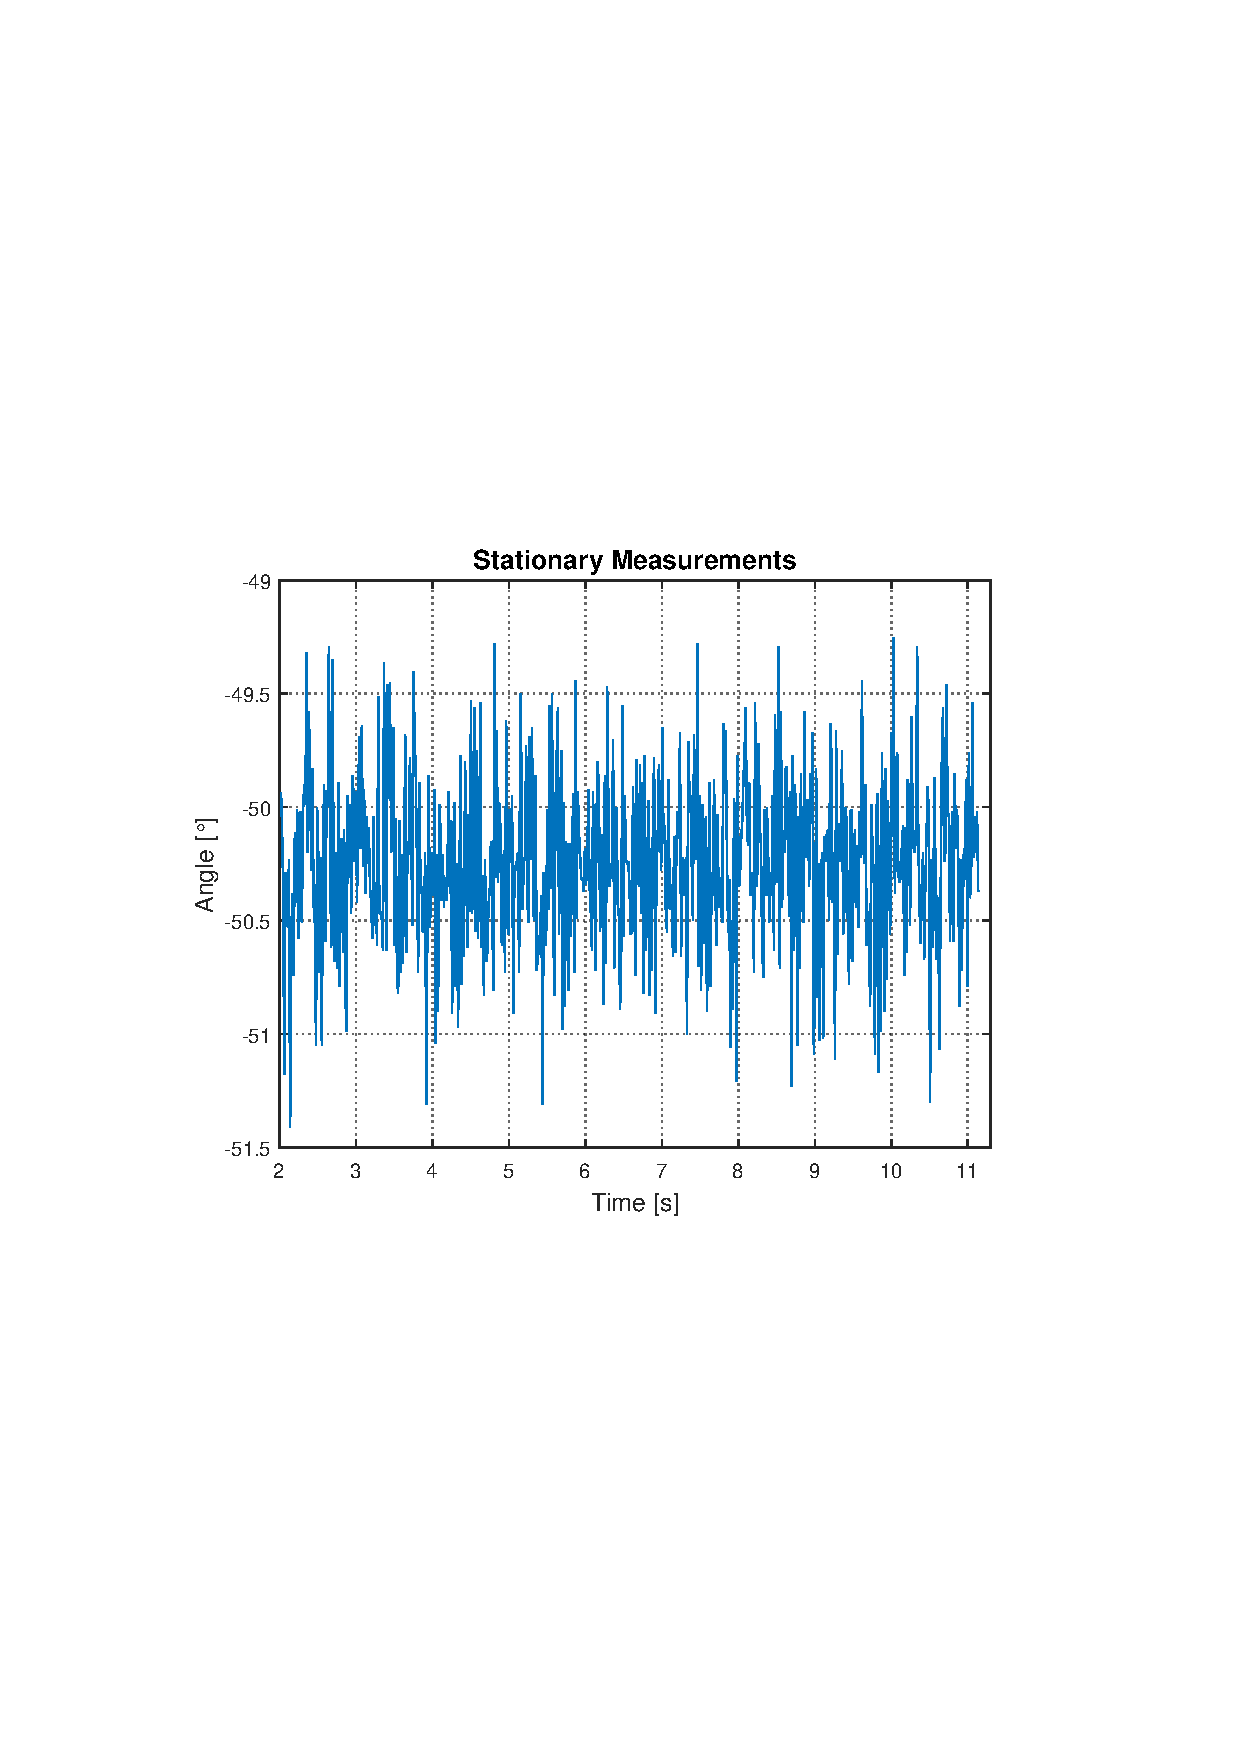
\includegraphics[width=1.1\textwidth]{figures/StationaryMeasurements.pdf}
  }
  \caption{A plot of data measured with the magnetometer while the vehicle is stationary. The x-axis indicates time and the y-axis is the angle.}
  \label{fig:StationaryMeasurementsMagnato}
\end{figure}

From \figref{fig:StationaryMeasurementsMagnato}, it can be seen how the angle measured vary with approximately 2 degrees. In the datasheet for the magnetometer it is explained that the sensor has a 1 to 2 degrees accuracy \cite{HMC5883L}, which is consistent with the measured data. To be able to analyse measured data affected by noise, an FFT is utilized. The FFT makes it possible to see the frequency components contained in the signal, thereby making it possible to find the signal and the noise affecting the signal. An FFT of the measured data is performed and illustrated in \figref{fig:StationaryMeasurementsMagnato}.

\begin{figure}[H]
  \centering
 	%Trim margins @:   left        bottom       right       top
 	\adjustbox{ trim = {.15\width} {.30\height} {.15\width} {.30\height}, clip }
  {
    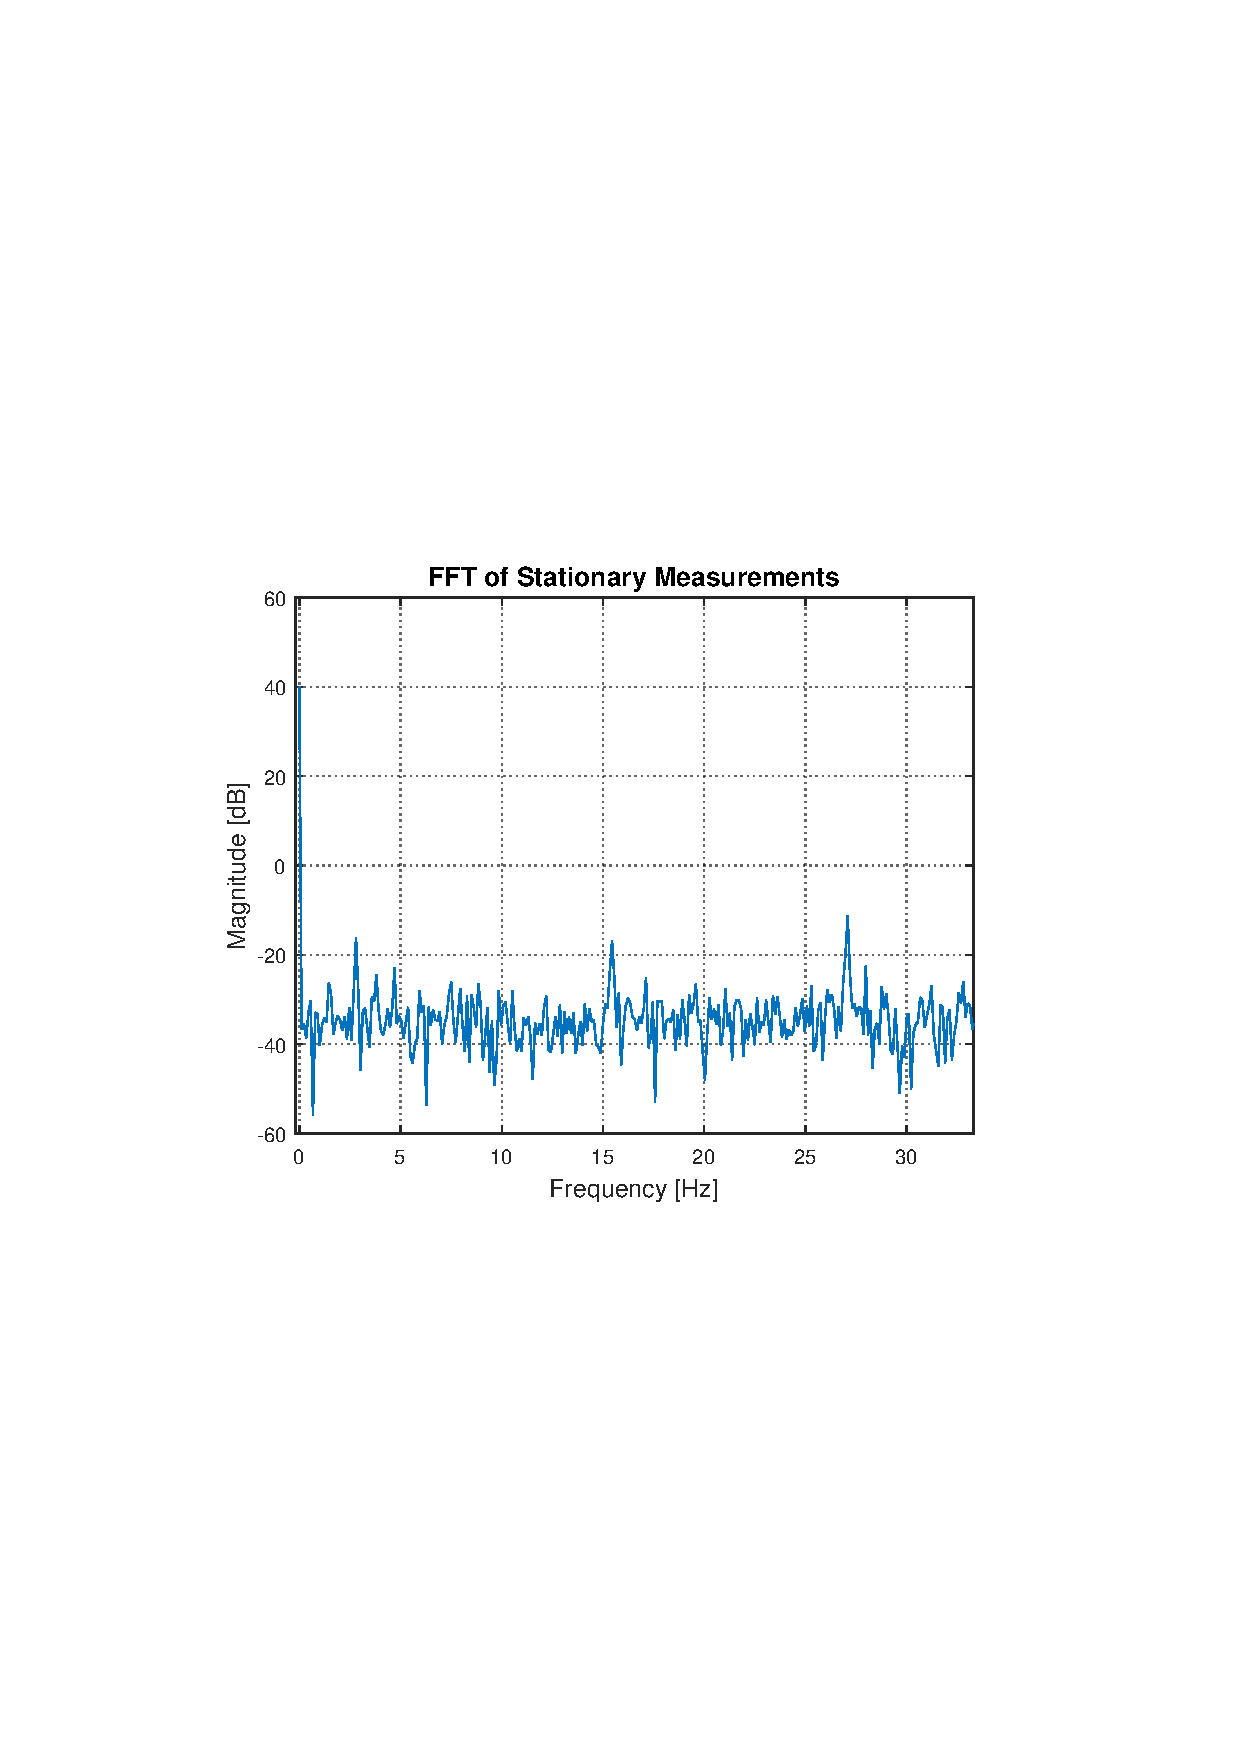
\includegraphics[width=1.1\textwidth]{figures/FFTofStationaryMeasurements.pdf}
  }
  \caption{A FFT of the measured data illustrated in \figref{fig:StationaryMeasurementsMagnato}}
  \label{fig:FFTofStationaryMeasurements}
\end{figure}

The data measured in \figref{fig:StationaryMeasurementsMagnato} is acquired with a sampling frequency of 66.6 \si{Hz}. The Nyquist-Shannon Sampling Theorem says that to find the frequency components contained in a signal, it is necessary to have at least twice the sampling frequency \cite{AVOppenheim}:
%
\begin{flalign}
\Omega_s &\geq 2 \cdot \Omega_N \unit{Hz}
\label{eq:Nyquistfrequency}
\end{flalign}
\hspace{6mm} Where:\\
\begin{tabular}{p{1cm}lll}
& \si{\Omega_s}            	& is the sampling frequency         &\unitWh{Hz} \\
& \si{\Omega_N}				& is the Nyquist frequency			&\unitWh{Hz} \\
\end{tabular}

This is illustrated in \figref{fig:FFTofStationaryMeasurements}, where the frequency components only goes from 0 to 33.3 Hz on the x-axis, which is half the sampling frequency. The y-axis is the magnitude of the frequency components of the signal.

From the FFT performed, as seen in \figref{fig:FFTofStationaryMeasurements}, a spike is present at 0 \si{Hz}. This is the DC value, i.e. the offset seen in \figref{fig:StationaryMeasurementsMagnato}. This frequency component is the signal which the filter should not attenuate. The frequency components present after 0 Hz, is the noise from the sensor. The noise is determined to be white noise, as it is looks evenly distributed over the frequency range.

Some considerations have to be made for the filter requirements, to ensure that the filter is not influencing the system and the desired frequency needlessly.

\subsection{Filter Type}
Data from the filter has been examined, it is thereby possible to examine which filter would be suitable for fulfilling the predetermined requirements. It should do this without influencing the DC-value and the system needlessly.

\begin{figure}[H]
	\centering
	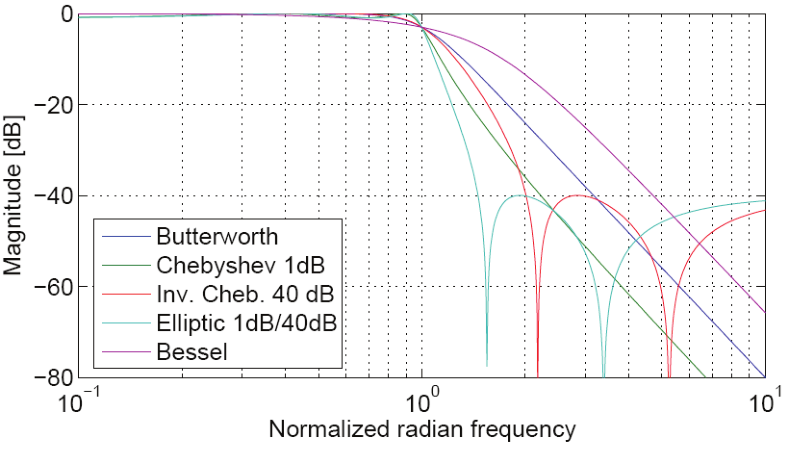
\includegraphics[scale=1]{figures/Filtertypes1.pdf}
	\caption{Frequency response for various filter types}
	\label{fig:Filtertype1}
\end{figure}

The disadvantages of a Elliptic filter is that it has both ripples in the pass- and stopband. additionally, it has a high group delay both before and at the cutoff frequency, this can be seen in \figref{fig:groupdelay}. The advantage of a Elliptic filter is that is has the sharpest cut-off frequency of the filters illustrated in \figref{fig:Filtertype1}.

The Chebyshev filter only has ripples in the passband, and a sharp cut-off frequency, but still has a high group delay before and at the cut-off frequency. The inverse Chebyshev only has ripples in the stopband, but does not have as sharp cut-off frequency as the Chebyshev and the Elliptic filter. Compared to the two former filter it has a lot less group delay before and after the cut-off frequency.

The Bessel filter has the lowest group delay before and at the cut-off frequency, see \figref{fig:groupdelay}. additionally, it does not have any ripples, neither in pass- or stopband. The disadvantage of the filter is it has the least sharpest cut-off frequency of the filters illustrated in \figref{fig:Filtertype1}.

The Butterworth filter has a sharper cut-off frequency compared to the Bessel filter and as the Bessel filter it does not have any ripples neither in the pass- or stopband. Furhtermore, the Butterworth filter has the second lowest group delay at the cut-off frequency compared to the other filters illustrated in \figref{fig:groupdelay}. 

\begin{figure}[H]
	\centering
	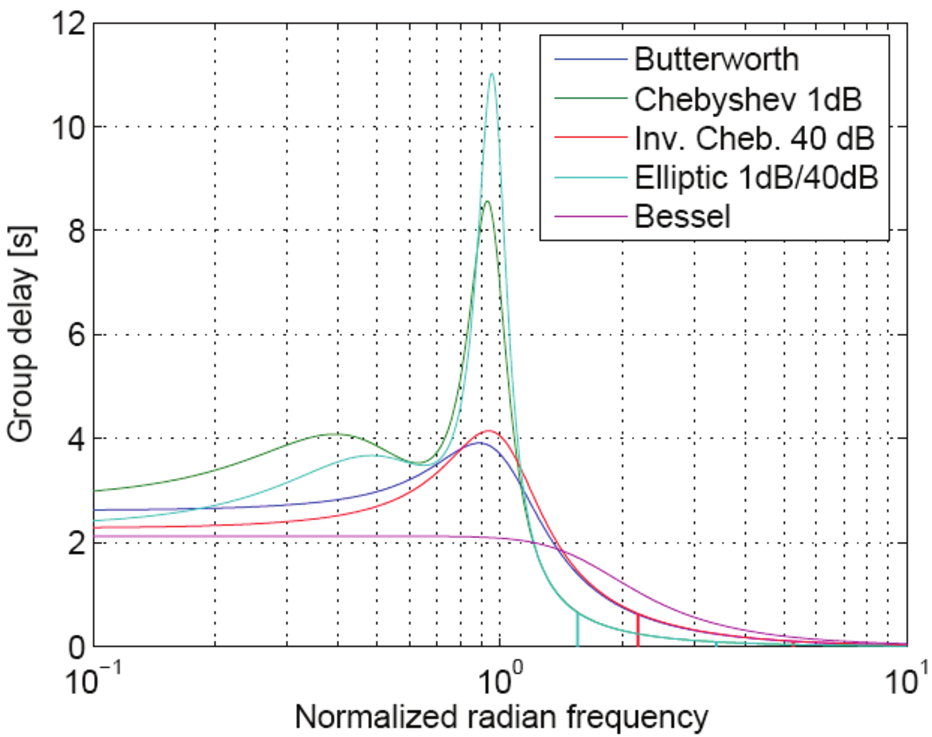
\includegraphics[scale=0.7]{figures/Filtertypes2.pdf}
	\caption{Frequency response illustrating group delay for various filter types}
	\label{fig:groupdelay}
\end{figure}

Because of the above-mentioned descriptions of the filters, a Butterworth filter has been selected for filtering the measured data. The Butterworth does not have any ripples in the passband which could influence the DC-value, seen in \figref{fig:FFTofStationaryMeasurements}, and compared to the other described filters, the Butterworth has a small group delay.

Considerations for the filter has been made, and it is thereby possible to specify the requirements for the filter.

\section{Filter Requirements} \label{sec:FilterRequirements}
From the filter considerations \secref{sec:FilterConsiderations}, it is possible to establish the specifications for the filter.

It has been decided to design a filter with a cut-off frequency which is less than one decade above the highest frequency pole. This will affect the system and cause a delay. To ensure the delay does not cause instability the filter first needs to be designed and simulated. Furthermore, since it is desired to influence the DC-signal as little as possible, see \figref{fig:FFTofStationaryMeasurements}, a low-pass filter is implemented.

By the use of and iterative process frequency requirements for the pass - and stopband has been established. A passband frequency of 19 \si{Hz} has been chosen. The ideal filter would have a passband attenuation of 0 \si{dB}. Since this is not a ideal filter a maximum attenuation variation is set from 1 \si{dB} to 0 \si{dB}. The stopband frequency has been chosen to 29 \si{Hz} with an attenuation of 40 \si{dB}.

Since the requirements needs to be adaptable to the z-plane, the Nyquist-Shannon sampling theorem \cite{AVOppenheim}, is utilized:
%
\begin{flalign}
\eq{\Omega_N}{\frac{2\pi \cdot f_s}{2}}
\end{flalign}
%
If 66.6 is said to be equal to \si{2\pi}, then the passband 19 \si{Hz} and the stopband 29 \si{Hz} will be equal to:
%
\begin{flalign}
\frac{19\pi}{33.3} &= 0.5705 \pi \quad \wedge \quad \frac{29\pi}{33.3} = 0.8709\pi
\end{flalign}
%
\textbf{Summary of Filter Specifications:}
%
\begin{itemize}
	\item \textbf{Filtertype}
		\begin{itemize}
			\item[] A Butterworth lowpass filter is designed.
		\end{itemize}
	\item \textbf{Passband specifications}
		\begin{itemize}
		 \item[] \si{0,08912 \leq |H(e^{j\omega})| \leq 1}
		 \item[] \si{0 \leq |\omega| \leq 0.5705 \pi}
		\end{itemize}
	\item \textbf{Stopband specifications}
		\begin{itemize}
		 \item[] \si{|H(e^{j\omega})| \leq 0,01}
		 \item[] \si{0.8709 \pi \leq |\omega| \leq \pi}
		\end{itemize}
\end{itemize}

The specifications for the filter is established, and it is thereby possible to design the filter.

\section{Design}
Various methods can be utilized when designing a digital filter. In the following subsection two methods for transferring a continuous-time filter to the z-domain is examined. The specific design process of the Butterworth low-pass filter will be done by following steps retrieved from \cite{AVOppenheim}.

\subsection{Bilinear Transform vs. Impulse Invariance transformation}
There is different methods for transferring a continuous-time filter to a discrete-time filter, the two most common transformation methods is examined. The first method of the two is the impulse invariance transformation.

When utilizing the impulse invariance transformation a discrete filter is generated by sampling a impulse response of a continuous analogue prototype filter. The impulse response of the discrete-time filter is proportional to the impulse response of the continuous-time filter with equally spaced samples, i.e.  making the discrete-filter from a sampled continuous-time prototype filter, \cite{AVOppenheim}.

This makes a linear mapping, \si{\omega = \Omega \cdot T_d} for each pole in the analogue filter's transfer function on the s-plane to a pole on the z-plane. 

The main issue when utilizing the impulse variance method is that the sampling rate needs to be relatively high compared to the filter's bandwidth, to not cause aliasing \cite{LyonsR.G}. In the frequency response, seen in \figref{fig:ImpulseVariantFrequencyResponse}, it can be seen that the response of a 6th-order Butterworth filter transformed by impulse invariance, has a frequency response which is larger than from 0 to \si{pi}, hence causing aliasing.

\begin{figure}[H]
	\centering
	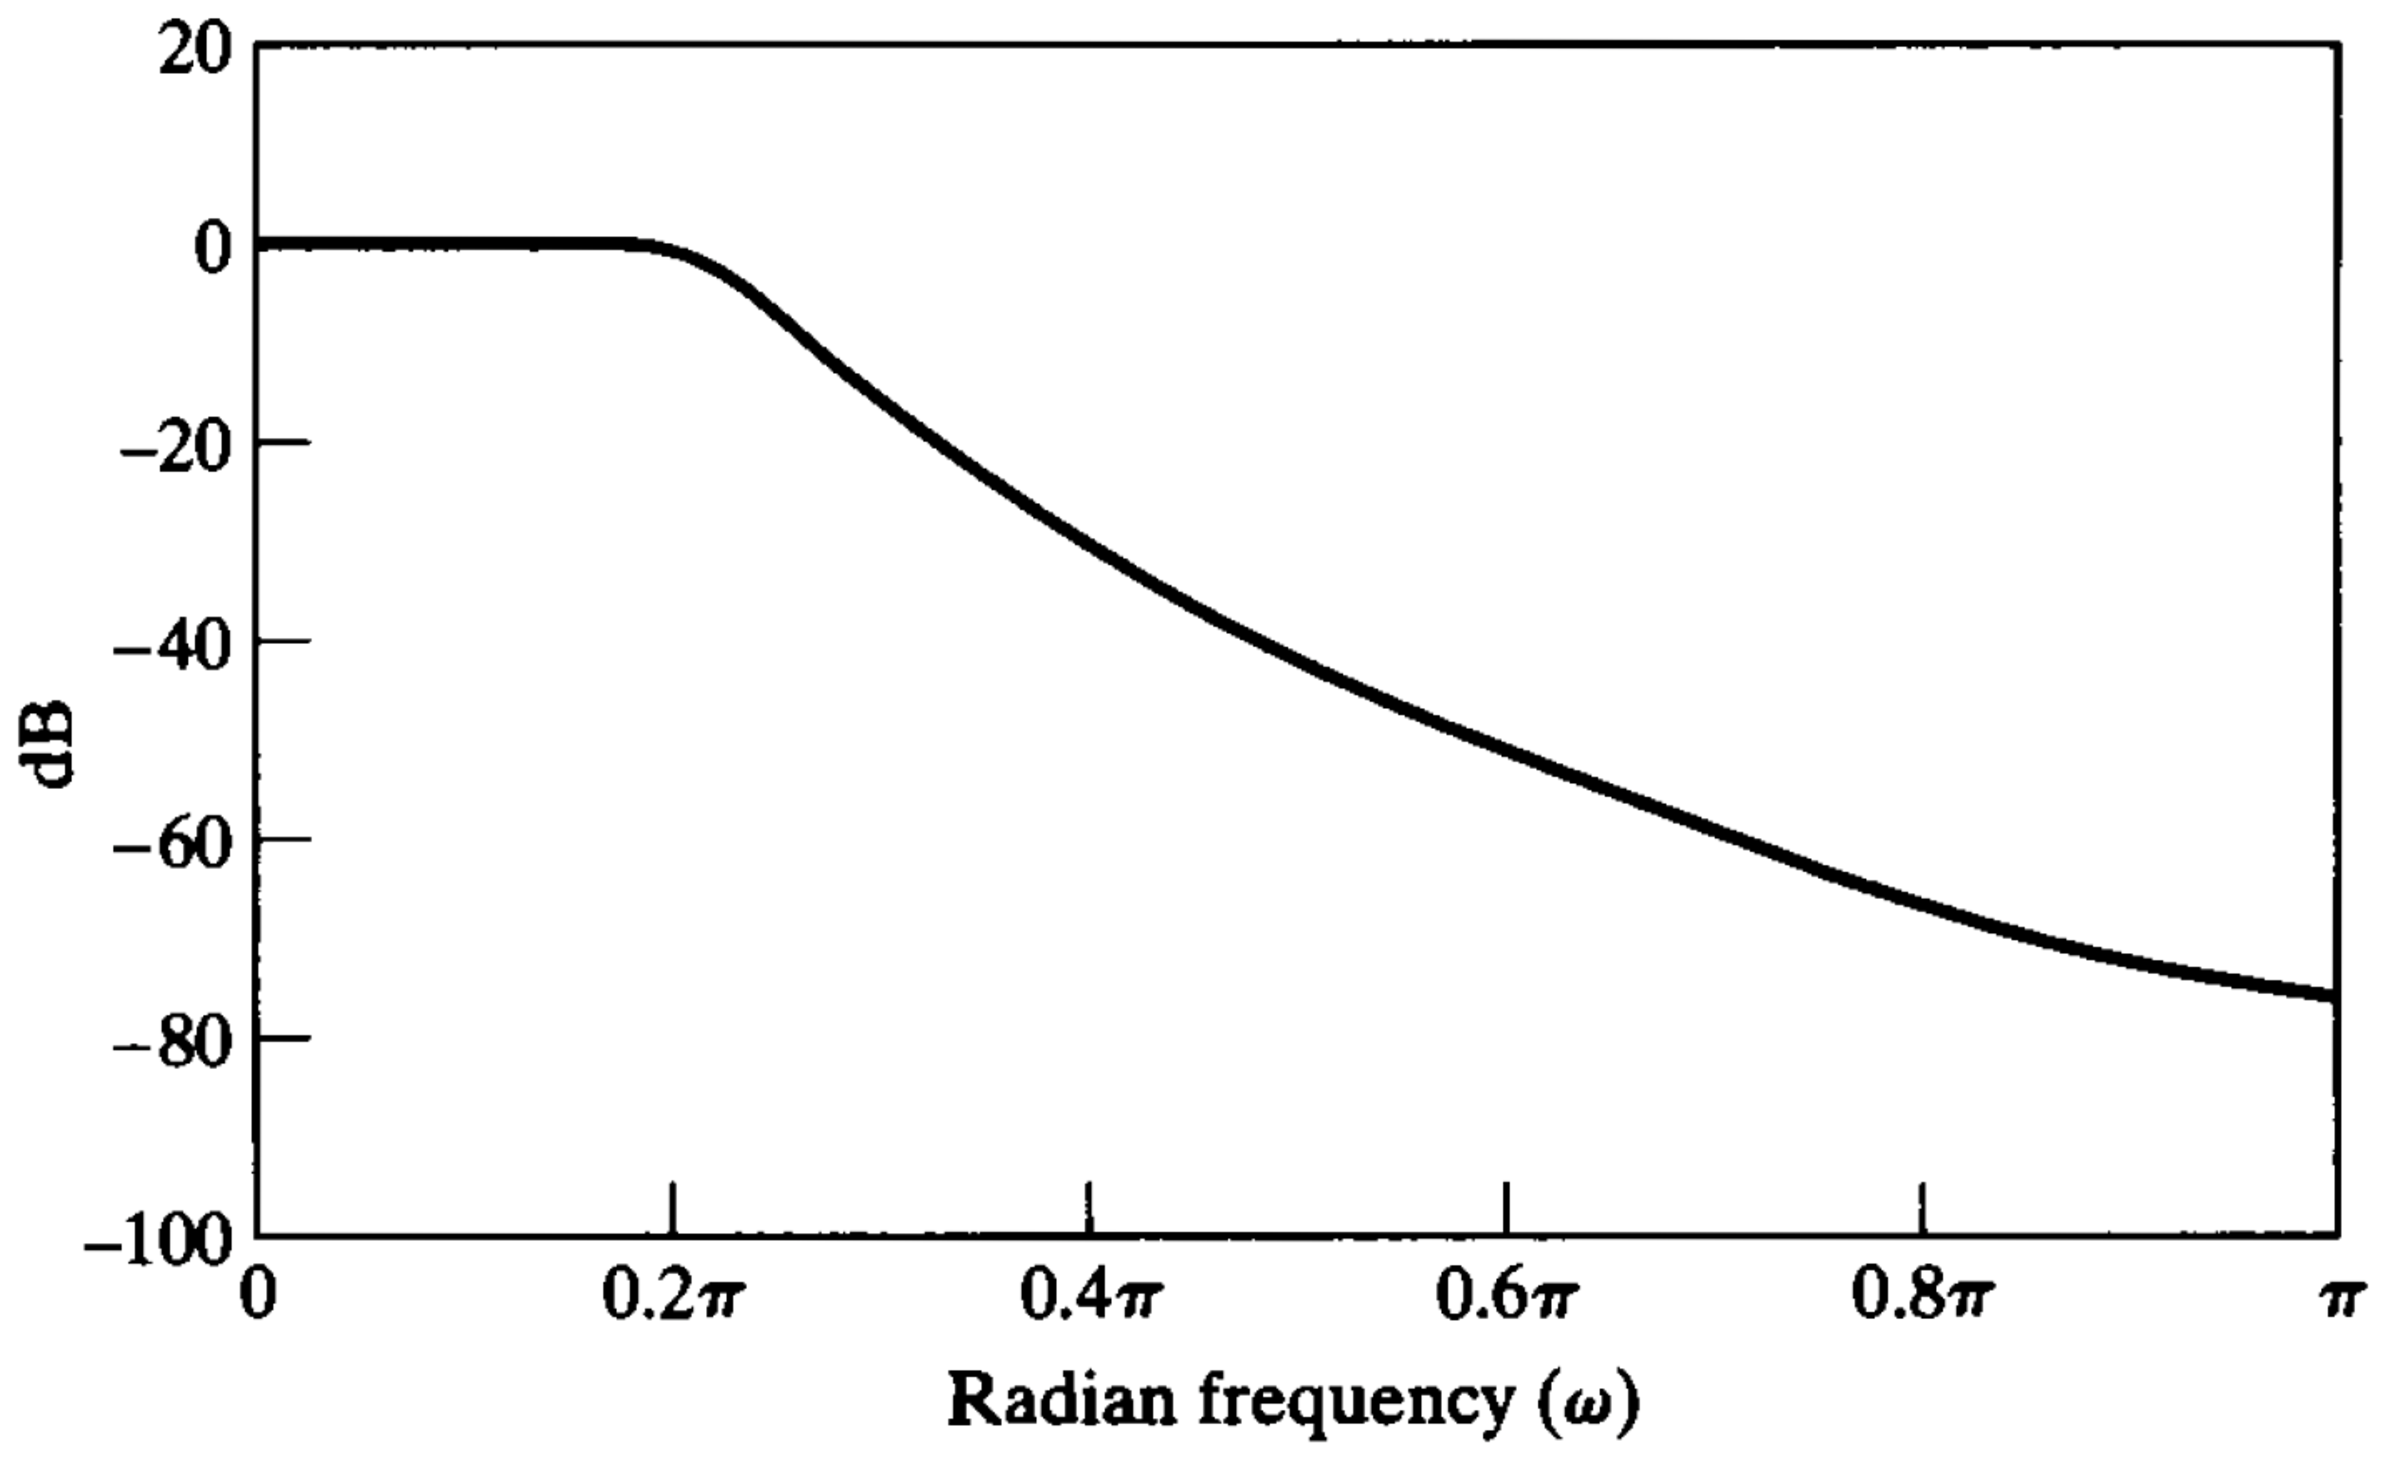
\includegraphics[scale=0.2]{figures/BilinearFrequencyResponse.pdf}
	\caption{A frequency response of a transformed impulse variance 6th order Butterworth filter \cite{AVOppenheim}.}
	\label{fig:ImpulseVariantFrequencyResponse}
\end{figure}

The Bilinear transform also utilize a analogue prototype filter to convert from s-domain to z-domain, when designing a digital filter. This transformation type is not a linear transformation from the s-domain to the z-domain, as it is with the impulse variance method. Instead it is a non-linear transformation which is mapping poles from \si{-\infty < \Omega < \infty} in the s-domain to \si{-\pi < \omega < \pi} in the z-domain \cite{AVOppenheim}. This yields the following relationship between the continuous-time frequencies to the discrete-time frequencies:
%
\begin{flalign}
\omega &= 2 \cdot \arctan(\frac{\Omega \cdot T_d}{2}) \wedge \Omega = \frac{2}{T_d} \cdot \tan(\frac{\omega}{2}) &
\label{eq:bilinearprewarp}
\end{flalign}
%
A frequency response, of the same filter as the frequency response for the impulse invariance, is illustrated in \figref{fig:BilinearFrequencyResponse}. The bilinear transform avoids aliasing problems because it maps the entire s-planes imaginary axis onto the z-planes unit circle \cite{AVOppenheim}. The s-plane and z-plane can be seen in \figref{fig:S-planeVsZ-plane}.
%
\begin{figure}[H]
	\centering
	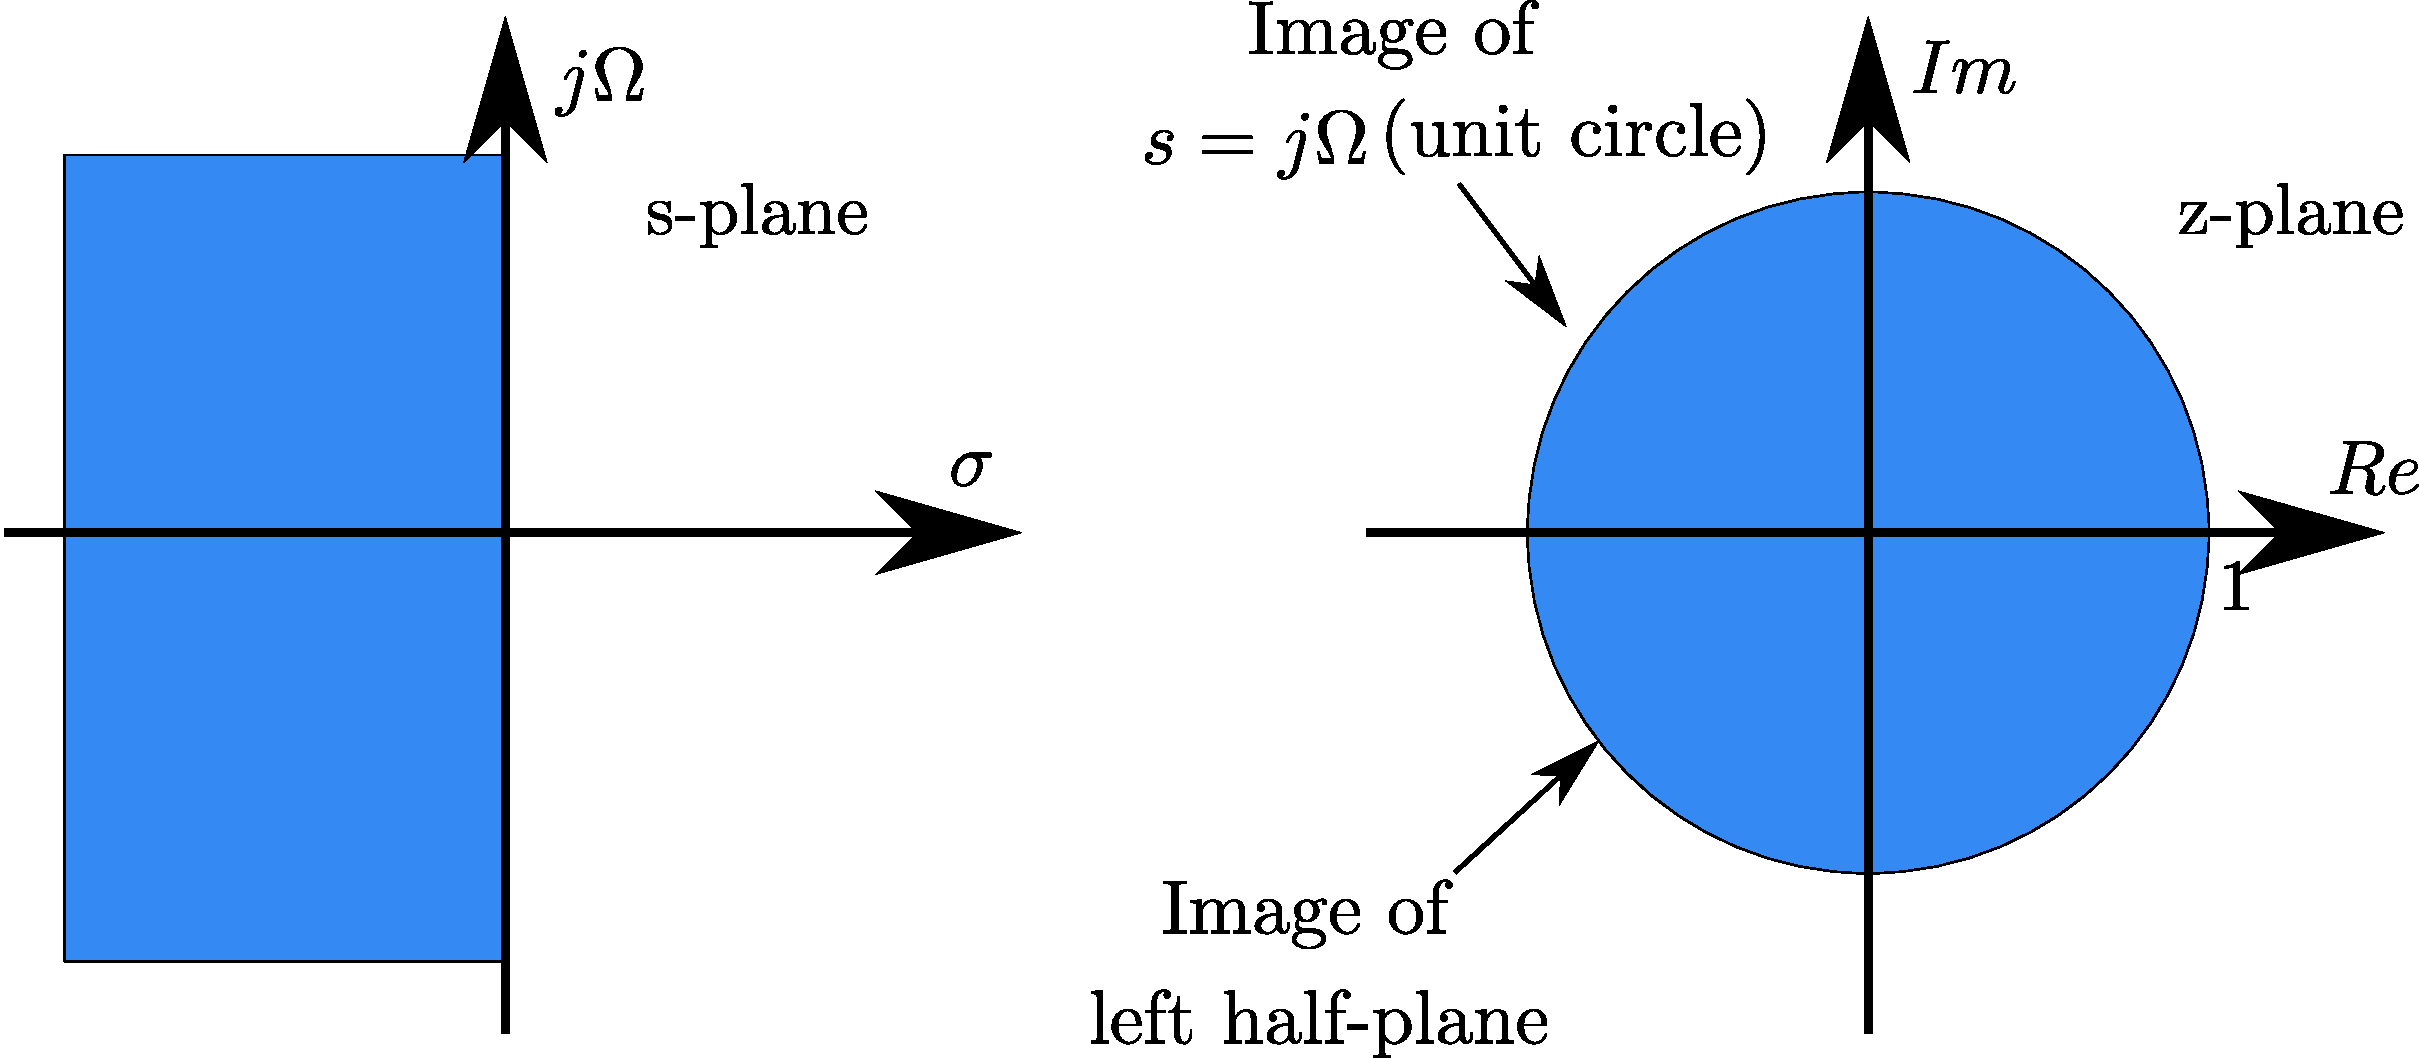
\includegraphics[scale=0.3]{figures/SplaneVsZplane.pdf}
	\caption{s-domain and z-domain \cite{AVOppenheim}.}
	\label{fig:S-planeVsZ-plane}
\end{figure}
%
From \figref{fig:BilinearFrequencyResponse} it can be seen that the frequency response does not exceed the limit from 0 to \si{\pi}, hence not causing a aliasing problem \cite{AVOppenheim}.

\begin{figure}[H]
	\centering
	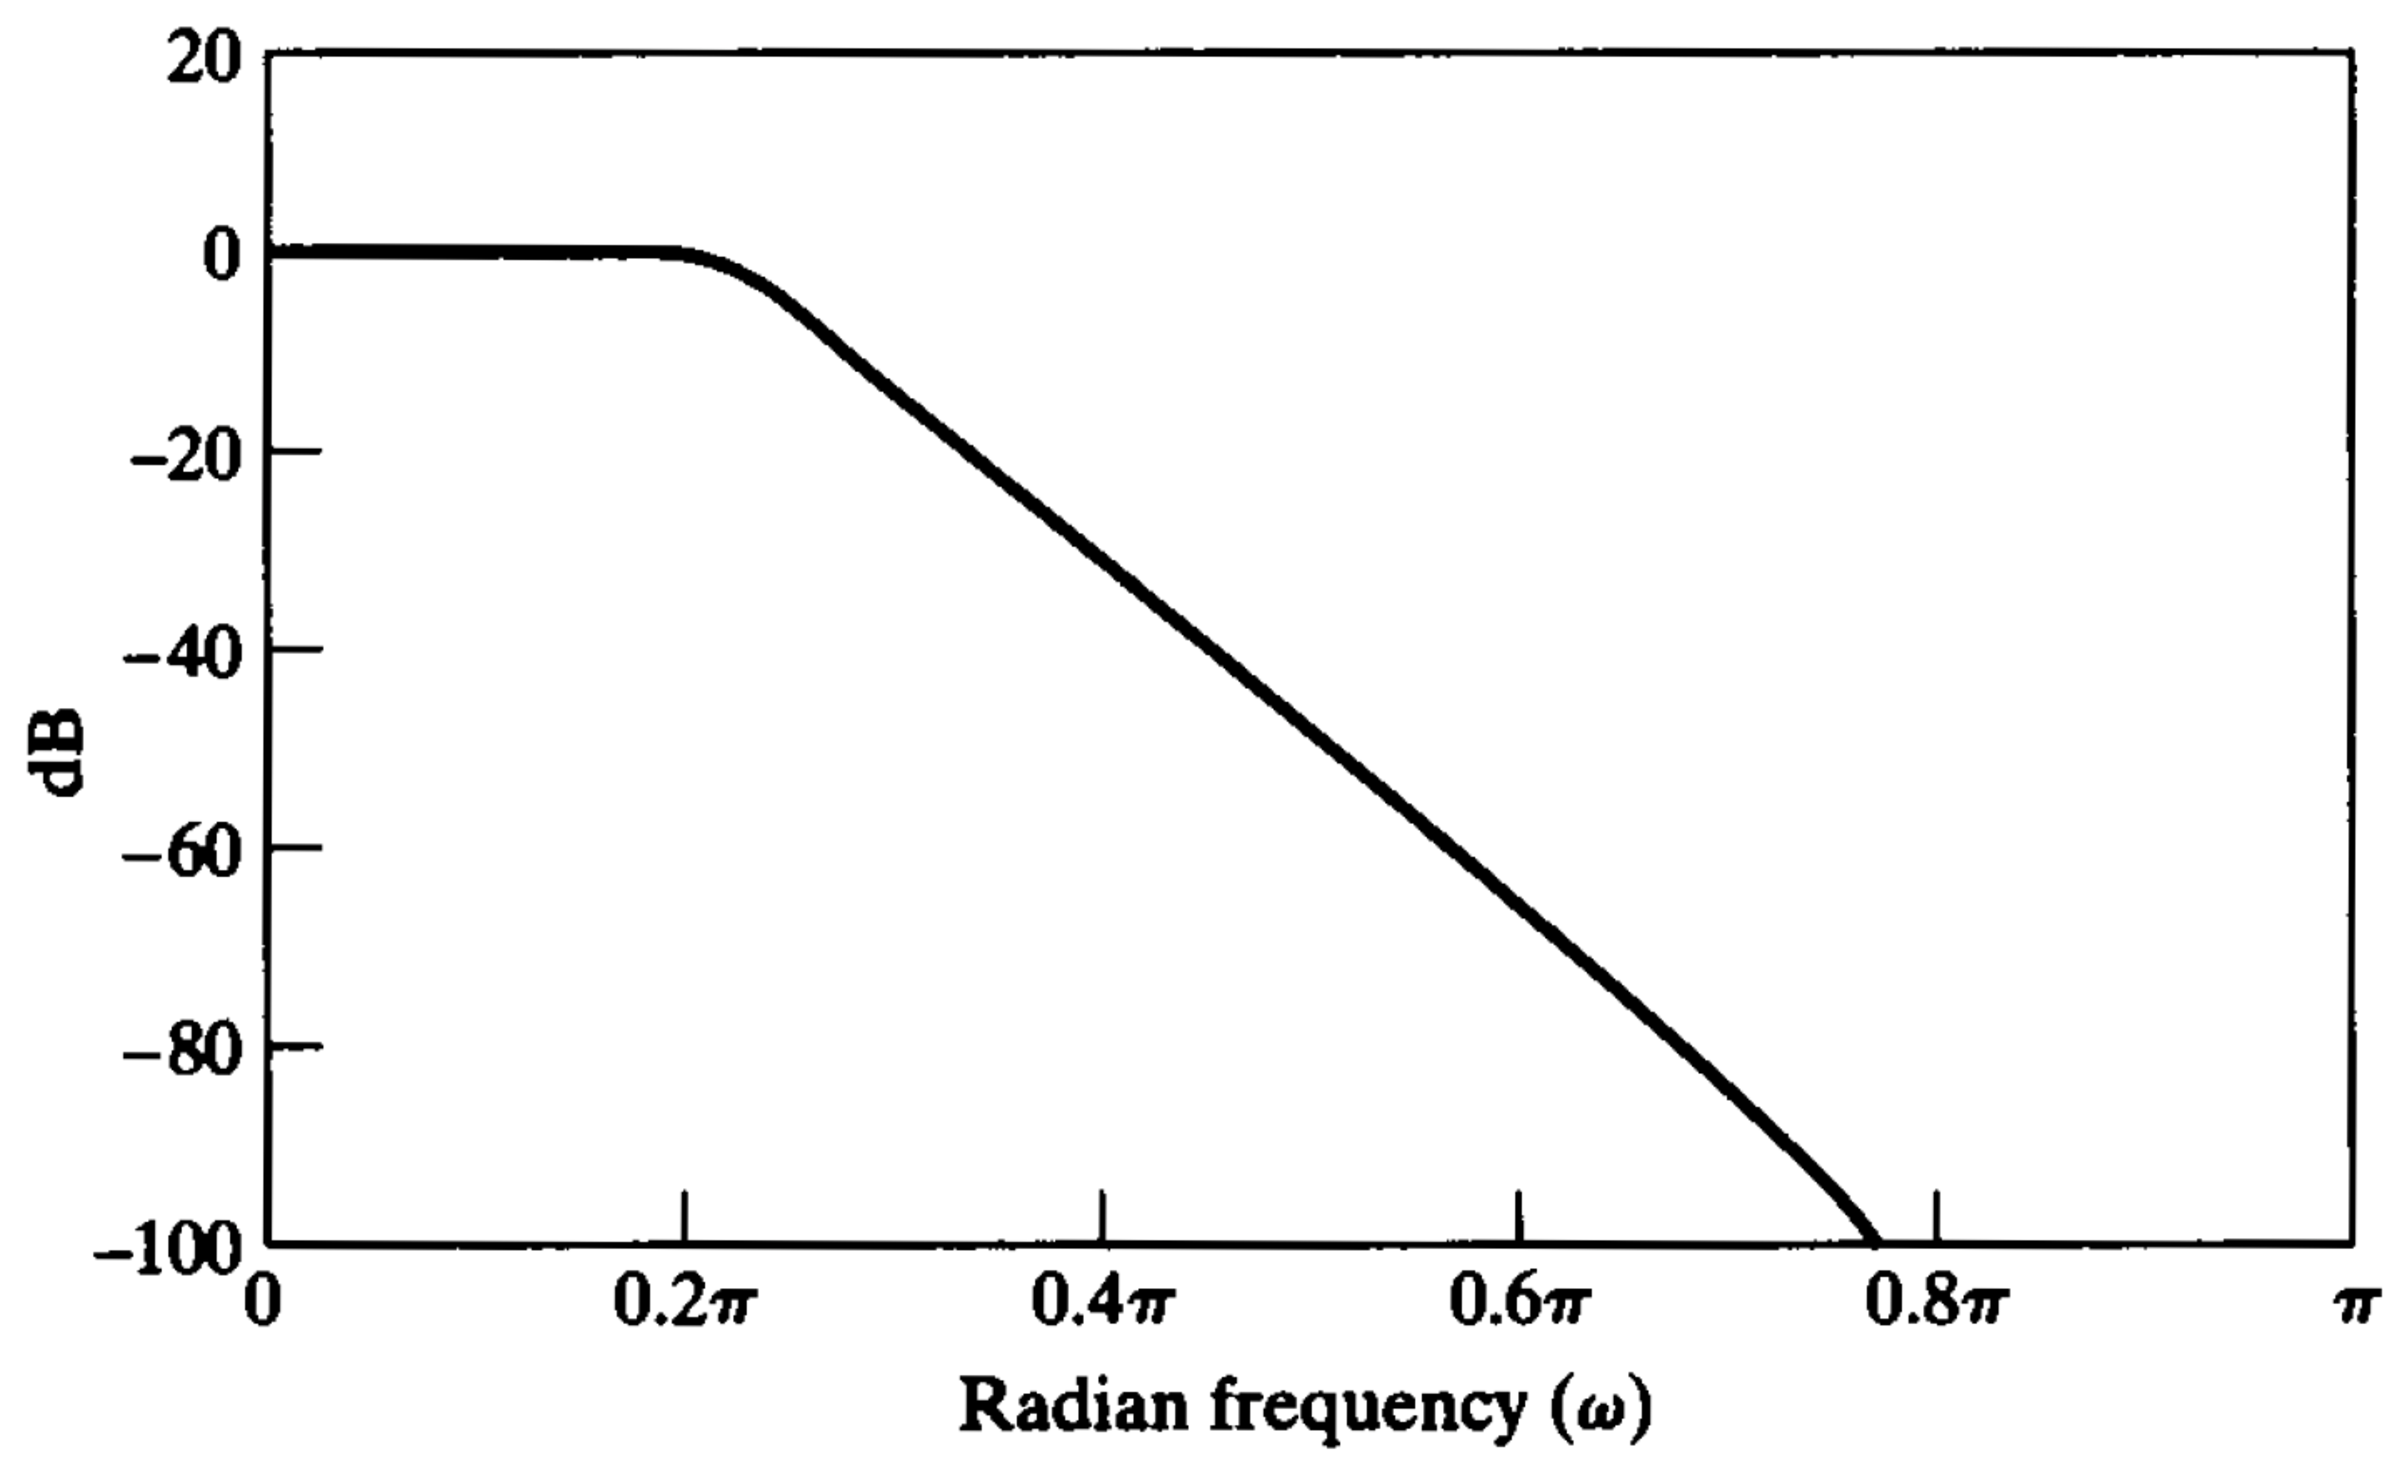
\includegraphics[scale=0.2]{figures/ImpulseVariantFrequencyResponse.pdf}
	\caption{A frequency response of a transformed bilinear transform 6th order Butterworth filter \cite{AVOppenheim}.}
	\label{fig:BilinearFrequencyResponse}
\end{figure}

It has been chosen to use the bilinear transformation when designing the filter. This is mainly due to the issue with aliasing that occurs when utilizing the impulse variance transform, which is avoided when utilizing the bilinear transform.

\subsection{Designing the Filter by the use of Bilinear Transform}
When utilizing bilinear transform it is necessary to frequency warp the passband frequency and the stopband frequency, from \secref{sec:FilterRequirements}. This is done by utilizing the relationship between the discrete-time frequencies in the z-domain to the continuous-time frequencies in the s-domain illustrated in \eqref{eq:bilinearprewarp}. 
%
\begin{flalign}
\Omega_p &= \frac{2}{0.015} \cdot \tan(\frac{0.5705 \pi}{2}) = 166 \quad \wedge \quad \Omega_s = \frac{2}{0.015} \cdot \tan(\frac{0.8709 \pi}{2}) = 644 \unit{Hz}
\label{eq:preqwardspecifications}
\end{flalign}
\hspace{6mm} Where:\\
\begin{tabular}{p{1cm}lll}
& \si{\Omega_p} & is the passband frequency in continuous time &\unitWh{Hz} \\
& \si{\Omega_s}	& is the stopband frequency in continuous time &\unitWh{Hz} \\
\end{tabular}

By utilizing the magnitude squared function for a Butterworth filter, it is possible to find the cut-off frequency:
%
\begin{flalign}
\eq{|H(e^{j\omega})|^2}{\frac{1}{1+(\frac{\Omega}{\Omega_c})^{2N}}}
\end{flalign}
\hspace{6mm} Where:\\
\begin{tabular}{p{1cm}lll}
& \si{\Omega}       & is the pre-warped frequencies  &\unitWh{Hz} \\
& \si{\Omega_c}		& is the cut-off frequency &\unitWh{Hz} \\
& \si{|H(e^{j\omega}|} & is the attenuation requirements set for the different bands from \secref{sec:FilterRequirements} &\unitWh{dB}
\end{tabular}

Since there is two unknown variables, the cut-off frequency and the order N, it is possible to calculate the values of these by utilizing the two equations with two unknowns:
%
 \begin{flalign}
0.89125^2 &= \frac{1}{1+(\frac{166}{\Omega_C})^{2N}} \quad \wedge \quad 0.01^2 = \frac{1}{1+(\frac{644}{\Omega_C})^{2N}}
\label{eq:OrderandCutoffFrequencyCON}
 \end{flalign}
%
The cut-off frequency is calculated to \textbf{197.9 \si{Hz}} and the order to 3.9, rounded to the nearest integer, i.e. \textbf{4}. When the order is known it is possible to utilize the following equation for finding the poles for a Butterworth filter.
%
\begin{flalign}
\eq{P_k}{\Omega_c \cdot e^{j(\frac{2 \cdot k -1}{2 \cdot N} \cdot \pi + \frac{\pi}{2})}}
\end{flalign}
%
Where k equal 1,2 \si{\dotsc N}.

Since it would desirable to have a stable system, the poles should only be located on the left side of the imaginary-axis.
%
\begin{flalign}
\eq{P_1}{\Omega_c \cdot e^{j \cdot \frac{5}{8} \pi}} \\
\eq{P_2}{\Omega_c \cdot e^{j \cdot \frac{7}{8} \pi}} \\
\eq{P_3}{\Omega_c \cdot e^{j \cdot \frac{9}{8} \pi}} \\
\eq{P_4}{\Omega_c \cdot e^{j \cdot \frac{11}{8} \pi}}
\end{flalign}
%
The poles placement indicated that it is two complex pole-pair, since they are symmetric around the real-axis.

The general transfer function for a Butterworth filter is defined as:
%
\begin{flalign}
\eq{H(s)}{\frac{G_o}{\prod\limits_{k = 1}^N (s-P_k)}}
\end{flalign}
\hspace{6mm} Where:\\
\begin{tabular}{p{1cm}lll}
& \si{G_o}       & is the gain of the filter  &\unitWh{\cdot} \\
\end{tabular}

The transfer function is rewritten to contain the located poles.

\begin{flalign}
\eq{H(s)}{\frac{G_o}{(s-\Omega_ce^{j\cdot \frac{5}{8} \cdot \pi})(s-\Omega_ce^{j\cdot \frac{7}{8} \cdot \pi})(s-\Omega_ce^{j\cdot \frac{9}{8} \cdot \pi})(s-\Omega_ce^{j\cdot \frac{11}{8} \cdot \pi})}}
\end{flalign}

Seen from the placement of the poles, and by the use of the rule \si{s = s*}, it is possible rewrite the transfer function.
%
\begin{flalign}
\eq{H(s)}{\frac{G_o}{(s-\Omega_ce^{j\cdot \frac{5}{8} \cdot \pi})(s-\Omega_ce^{j\cdot \frac{7}{8} \cdot \pi})(s-\Omega_ce^{-j\cdot \frac{7}{8} \cdot \pi})(s-\Omega_ce^{-j\cdot \frac{5}{8} \cdot \pi})}}
\end{flalign}
%
The transfer function is rewritten to contain the complex poles in standard form:
%
\begin{flalign}
\eq{H(s)}{\frac{G_o}{(s^2 + 2 \cdot \cos{(\frac{7}{8} \cdot \pi)} \cdot \Omega_c \cdot s + \Omega_c^2)(s^2 + 2 \cdot \cos{(\frac{5}{8} \cdot \pi)} \cdot \Omega_c \cdot s + \Omega_c^2)}}
\end{flalign}
%
The DC gain, \si{G_o} is determined by setting s to 0. furthermore, since you have 0 \si{dB} at DC which corresponds to 1 in amplitude, then \si{H(0)} is equal to 1. The DC gain will thereby be:
%
\begin{flalign}
\eq{G_o}{\Omega_c^4}
\end{flalign}
%
All the coefficients has been found for the transfer function, thus making it possible to perform a frequency response illustrated in \figref{fig:Continuoustimebodeplot}. The continuous transfer function will thereby be:
%
\begin{flalign}
\eq{H(s)}{\frac{\Omega_c^4}{(s^2 + 2 \cdot \cos{(\frac{7}{8} \cdot \pi)} \cdot \Omega_c \cdot s + \Omega_c^2)(s^2 + 2 \cdot \cos{(\frac{5}{8} \cdot \pi)} \cdot \Omega_c \cdot s + \Omega_c^2)}}
\label{eq:continuousTransfer}
\end{flalign}
%
\begin{figure}[H]
  \centering
 	%Trim margins @:   left        bottom       right       top
 	\adjustbox{ trim = {.15\width} {.30\height} {.15\width} {.30\height}, clip }
  {
    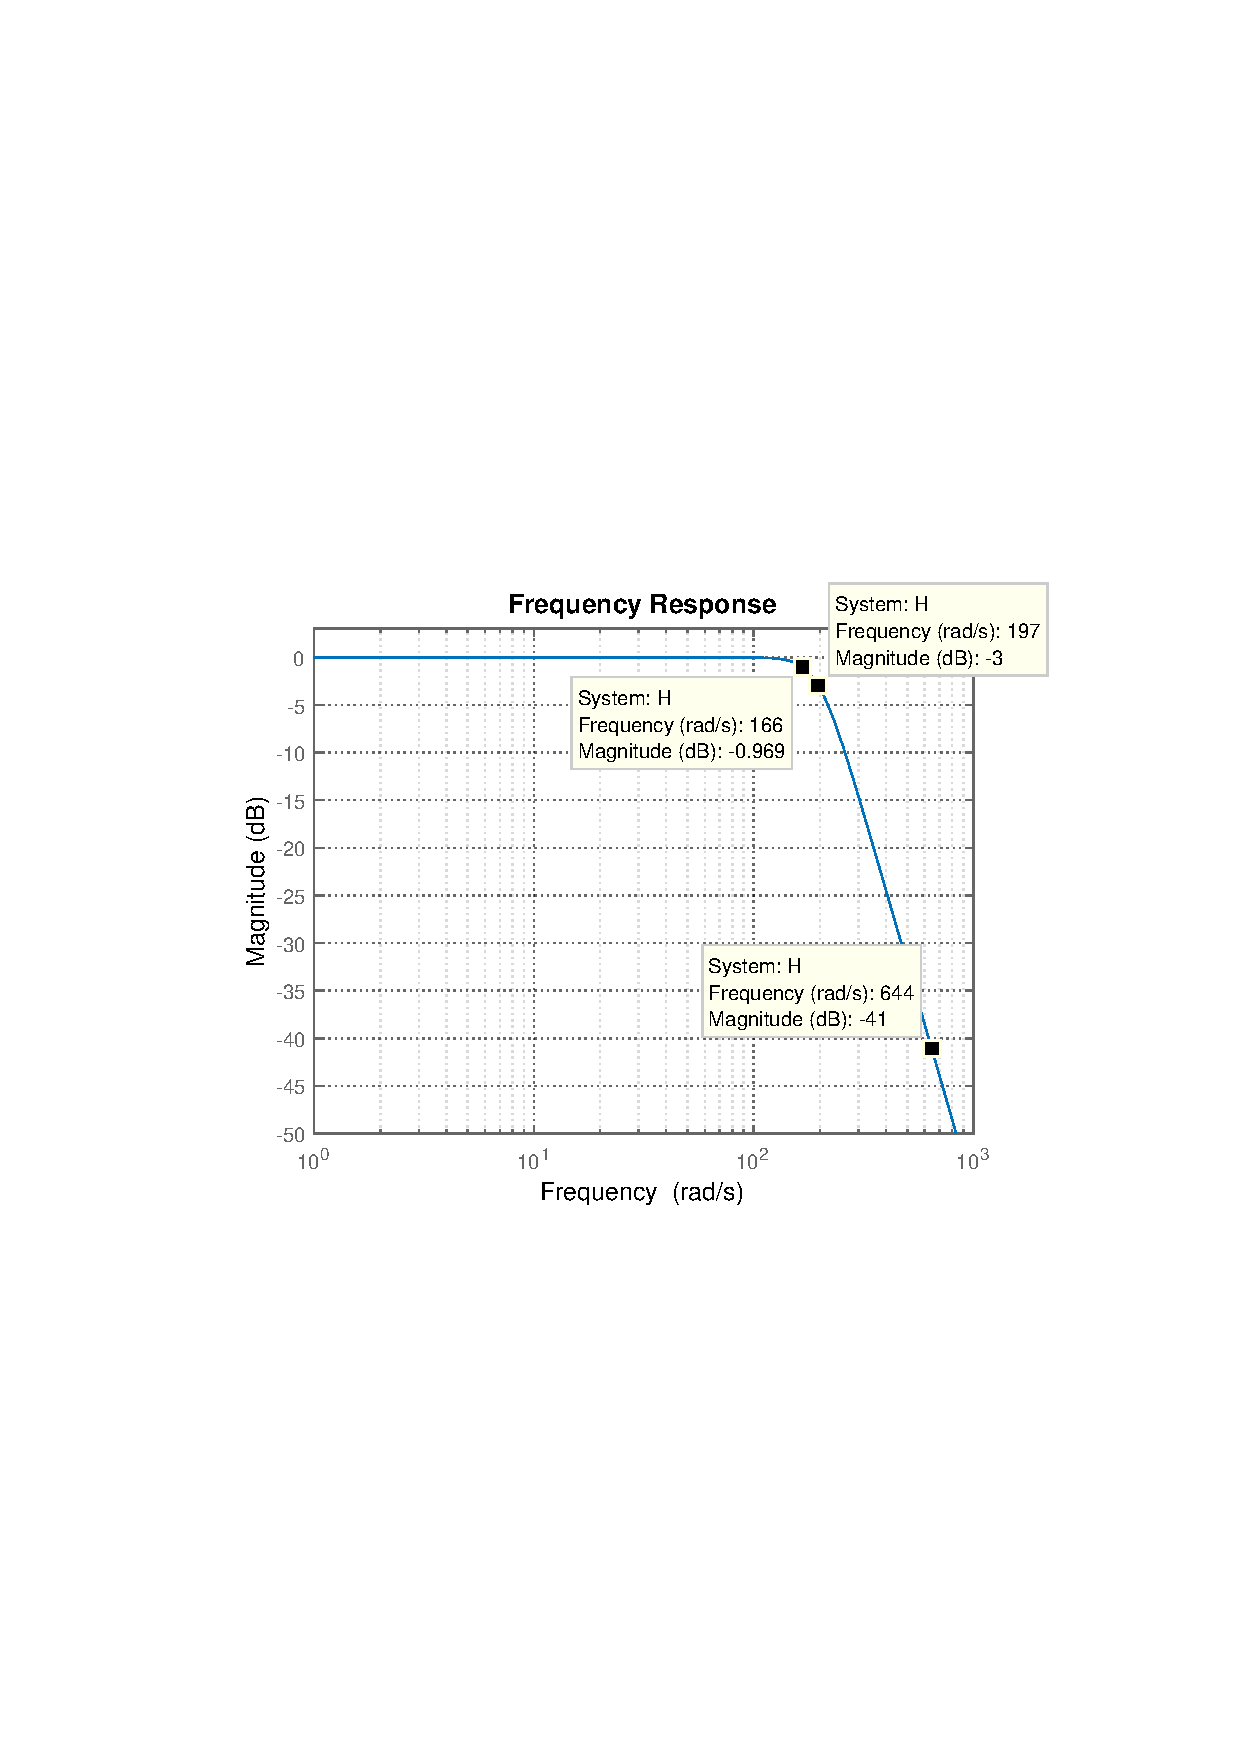
\includegraphics[width=1.1\textwidth]{figures/ContinusFilterResponse.pdf}
  }
  \caption{Bode plot of the continuous filter}
  \label{fig:Continuoustimebodeplot}
\end{figure}
%
The discrete specifications pre-warped to continuous-time, see \eqref{eq:preqwardspecifications}, is determined for the passband frequency to 166 \si{Hz} and for the stopband to \si{644}. Furthermore from the requirements set in \secref{sec:FilterRequirements}, the attenuation in the passband should be beneath 1 \si{dB} and the stopband should be at a attenuation of 40 \si{dB}. This requirements is in compliance with what is observed on \figref{fig:Continuoustimebodeplot}. Additionally, the cut-off frequency calculated in \eqref{eq:OrderandCutoffFrequencyCON} corresponds with what is illustrated in the frequency response.

The established continuous-time filter can now be transferred to the z-domain.

\subsection{Transforming the filter to the discrete-time domain}
The bilinear transform is utilized to transform the continuous-time filter to the z-domain. Substituting the expression for s, given in \eqref{eq:ssubz}, in the continuous-time transfer function, in \eqref{eq:continuousTransfer}, a discrete-time transfer function for the filter is determined.
%
\begin{flalign}
\eq{s}{\frac{2}{T_d}\left(\frac{1-z^{-1}}{1+z^{-1}}\right)}
\label{eq:ssubz}
\end{flalign}
%
A frequency response of the discrete-time transfer function is illustrated in \figref{fig:discretetimebodeplot}.

\begin{figure}[H]
  \centering
 	%Trim margins @:   left        bottom       right       top
 	\adjustbox{ trim = {.15\width} {.30\height} {.15\width} {.30\height}, clip }
  {
    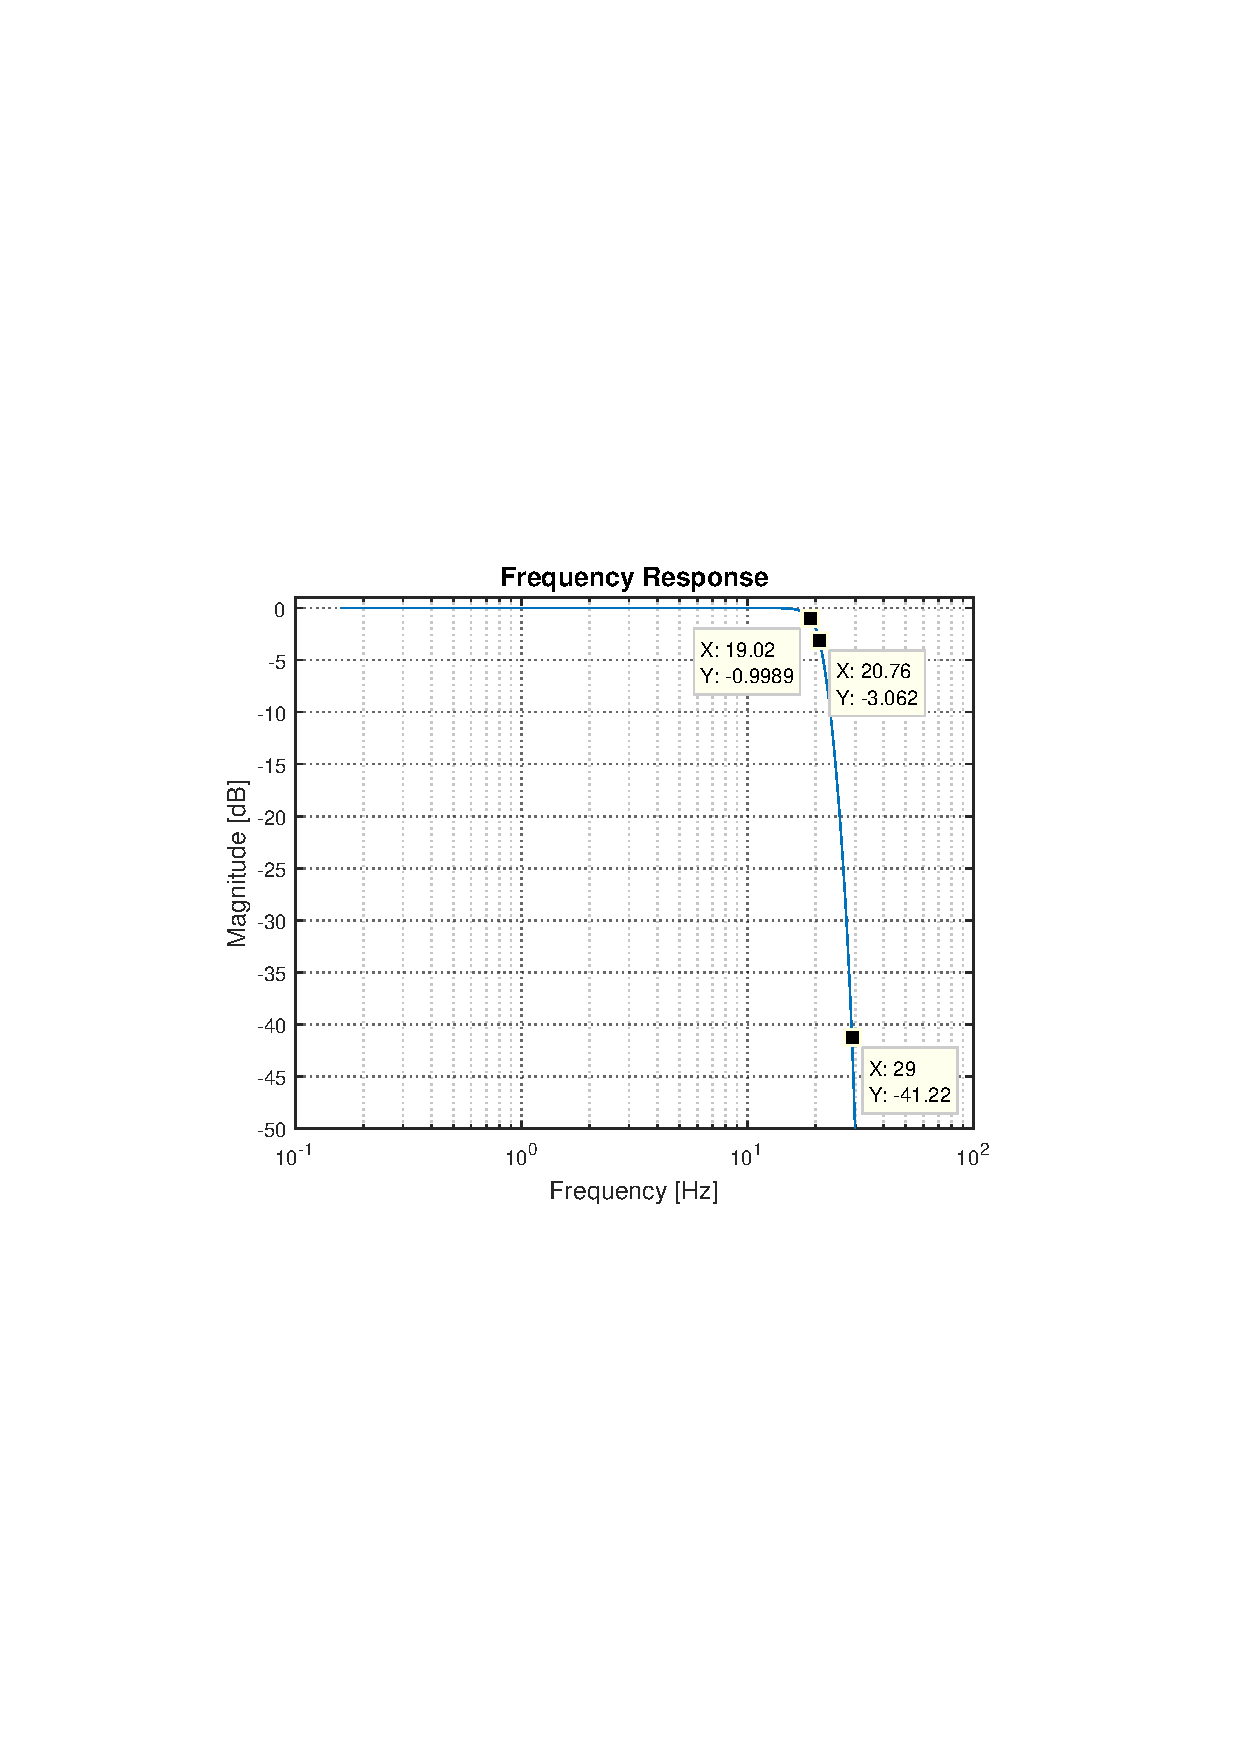
\includegraphics[width=1.1\textwidth]{figures/DiscreteFrequencyResponse.pdf}
  }
  \caption{Bode plot of the discrete time filter}
  \label{fig:discretetimebodeplot}
\end{figure}

The requirements set for the filter in \secref{sec:FilterRequirements} is in compliance with the frequency response plotted in \figref{fig:discretetimebodeplot}. The passband frequency should be at 19 \si{Hz} and the stopband at 29 \si{Hz}. Additionally, the attenuation in the passband within the range from 0 to 1 \si{dB} and the stopband attenuation of 40 \si{dB}.

By utilizing normalize expansion\todo{what's that?} it is possible to rewrite the discrete-time transfer function to a standard form, defined as:
%
\begin{flalign}
H(z) &= \frac{B(z)}{A(z)} = \frac{\smashoperator[r]{\sum_{n=0}^{M}} b_nz^{-n}}{\smashoperator[r]{\sum_{n=0}^{N}} a_nz^{-n}} =\frac{b_0 + b_1z^{-1} + b_2z^{-2} + \dotsc + b_Nz^{-M}}{1 + a_1z^{-1} + a_2z^{-2} + \dotsc + a_Mz^{-N}}
\end{flalign}
%
The coefficients, \si{a_N} and \si{b_M}, can be used directly when implementing the filter. The discrete transfer form is rewritten to:
%
\begin{flalign}
H(z) &= \frac{B(z)}{A(z)} = \frac{0.1882 + 0.7527z^{-1} + 1.129z^{-2} + 0.7527z^{-3} + 0.1882z^{-4}}{1 + 0.9595z^{-1} + 0.7785z^{-2} + 0.2358z^{-3} + 0.03691z^{-4}}
\label{eq:ImplementationCoefficients}
\end{flalign}
%
Where \si{a_0 = 1}.\todo{poof! numbers out of nowhere?}
\section{Implementation}
There is different methods to implement a IIR filter. The coefficients from \eqref{eq:ImplementationCoefficients}, can either be implemented directly by utilizing the structure called Direct form I or implemented with the structure Direct form II which has less delay. Compared to Direct form II, Direct form I has twice the delay. The fourth order low-pass Butterworth IIR filter in direct form II is illustrated in \figref{fig:IIRfilter}.
%
\begin{figure}[H]
	\centering
	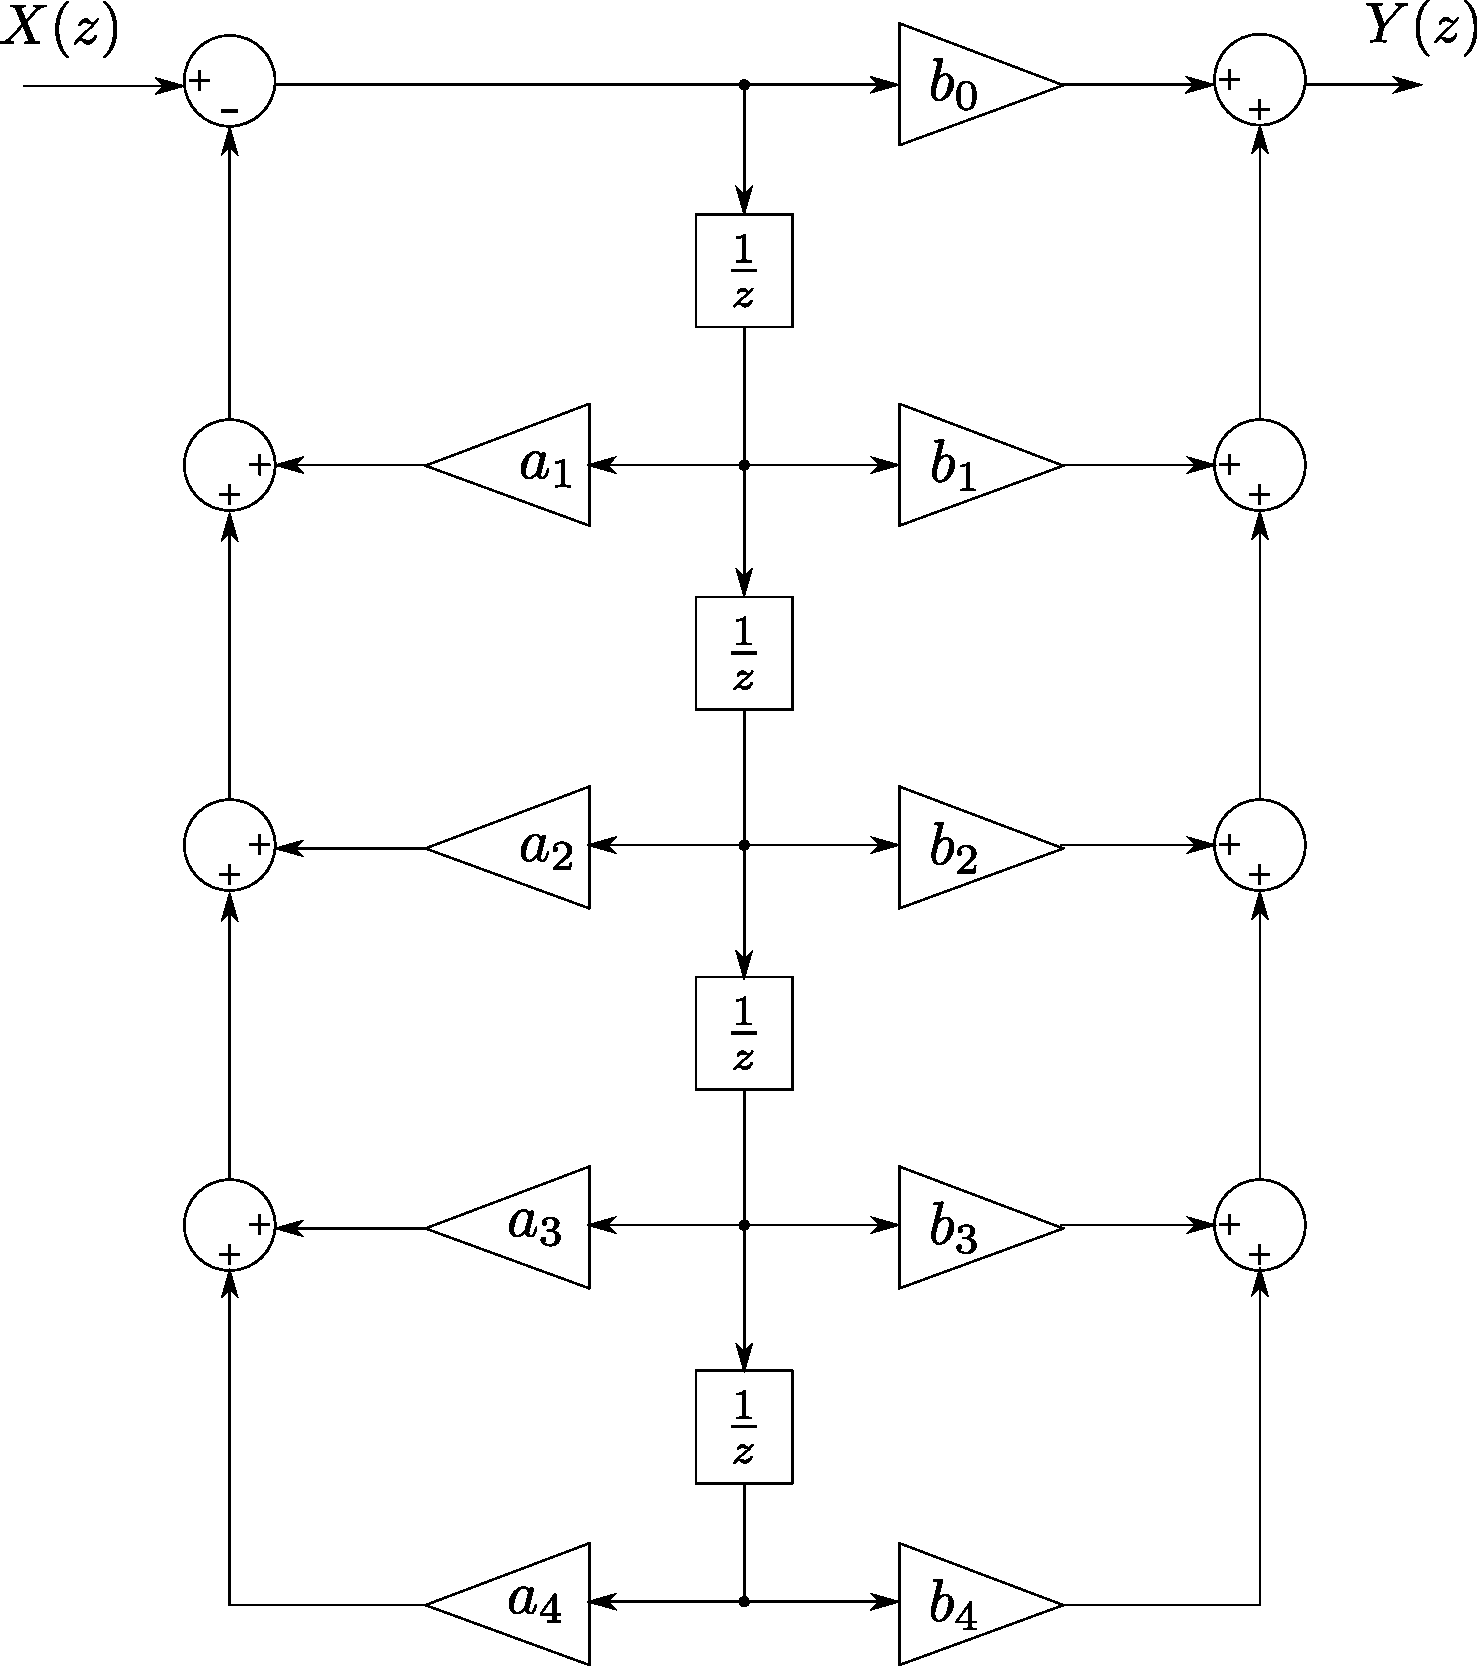
\includegraphics[scale=0.5]{figures/IIRfilter.pdf}
	\caption{fourth order low-pass Butterworth IIR filter implemented with the structure Direct form II}
	\label{fig:IIRfilter}
\end{figure}
%
By directly utilizing the structure and patterns of \figref{fig:IIRfilter}, it is possible to implement the filter almost directly in Matlab. The implementation of the related code can be seen in \autoref{lst:FilterMatlabImplementation}.
%
\lstset{language=Matlab, caption={Butterworth low-pass IIR filter Implementation in Matlab by the utilizing the Direct form II structure}, label=lst:FilterMatlabImplementation}
\begin{lstlisting}
for i = 1:707 %Quantity of samples

  Buffer0 = Input(i) - (a1*BUF1 + a2*BUF2 + a3*BUF3 + a4*BUF4) 
  %Calculated value of the first Buffer in Direct form II
	
  Output(i) = BUF0*b0 + b1*BUF1 + b2*BUF2 + b3*BUF3 + b4*BUF4 
  %The generated output of the filter
    	
  Buffer4 = Buffer3	%A delay generated by shifting the buffers
  Buffer3 = Buffer2
  Buffer2 = Buffer1
  Buffer1 = Buffer0
    
 end
\end{lstlisting}\todo{is this right? Shouldn't BUF1..4 be Buffer1..4?}

When implementing the code directly on a microcontroller a for-loop will not be utilized, as each sample from the Magnetometer is processed immediately, thus generating a filtered measurement for the control loop to utilize.
Buffer0 is located just above the first delay, \si{\frac{1}{z}}, in \figref{fig:IIRfilter}, Buffer1 beneath the first delay etc.. Buffer0 contains the Input, the measurement delivered by the magnetometer, substracted with the \si{a_N} coefficients from \eqref{eq:ImplementationCoefficients} multiplied with the related buffers.

Buffer0 now contains the needed information of the first part of the structure and can be utilized to transfer this value to be part the output. The output of the filter, i.e. the filtered measurement, is composed of the \si{b_M} coefficients and the related buffers. The delay needed is generated by shifting the value of the buffers.

\section{Results}
The filter is implemented in Matlab, and it is thereby possible to filter the measurements received from the Magnetometer, see \figref{fig:StationaryMeasurementsMagnato}, to see if the filter can decrease the sensors variations of approximately 2 degrees. The original measurements and the related filtered measurements is illustrated in \figref{fig:FinalImplementedFilter}.
%
\begin{figure}[H]
  \centering
 	%Trim margins @:   left        bottom       right       top
 	\adjustbox{ trim = {.15\width} {.30\height} {.15\width} {.30\height}, clip }
  {
    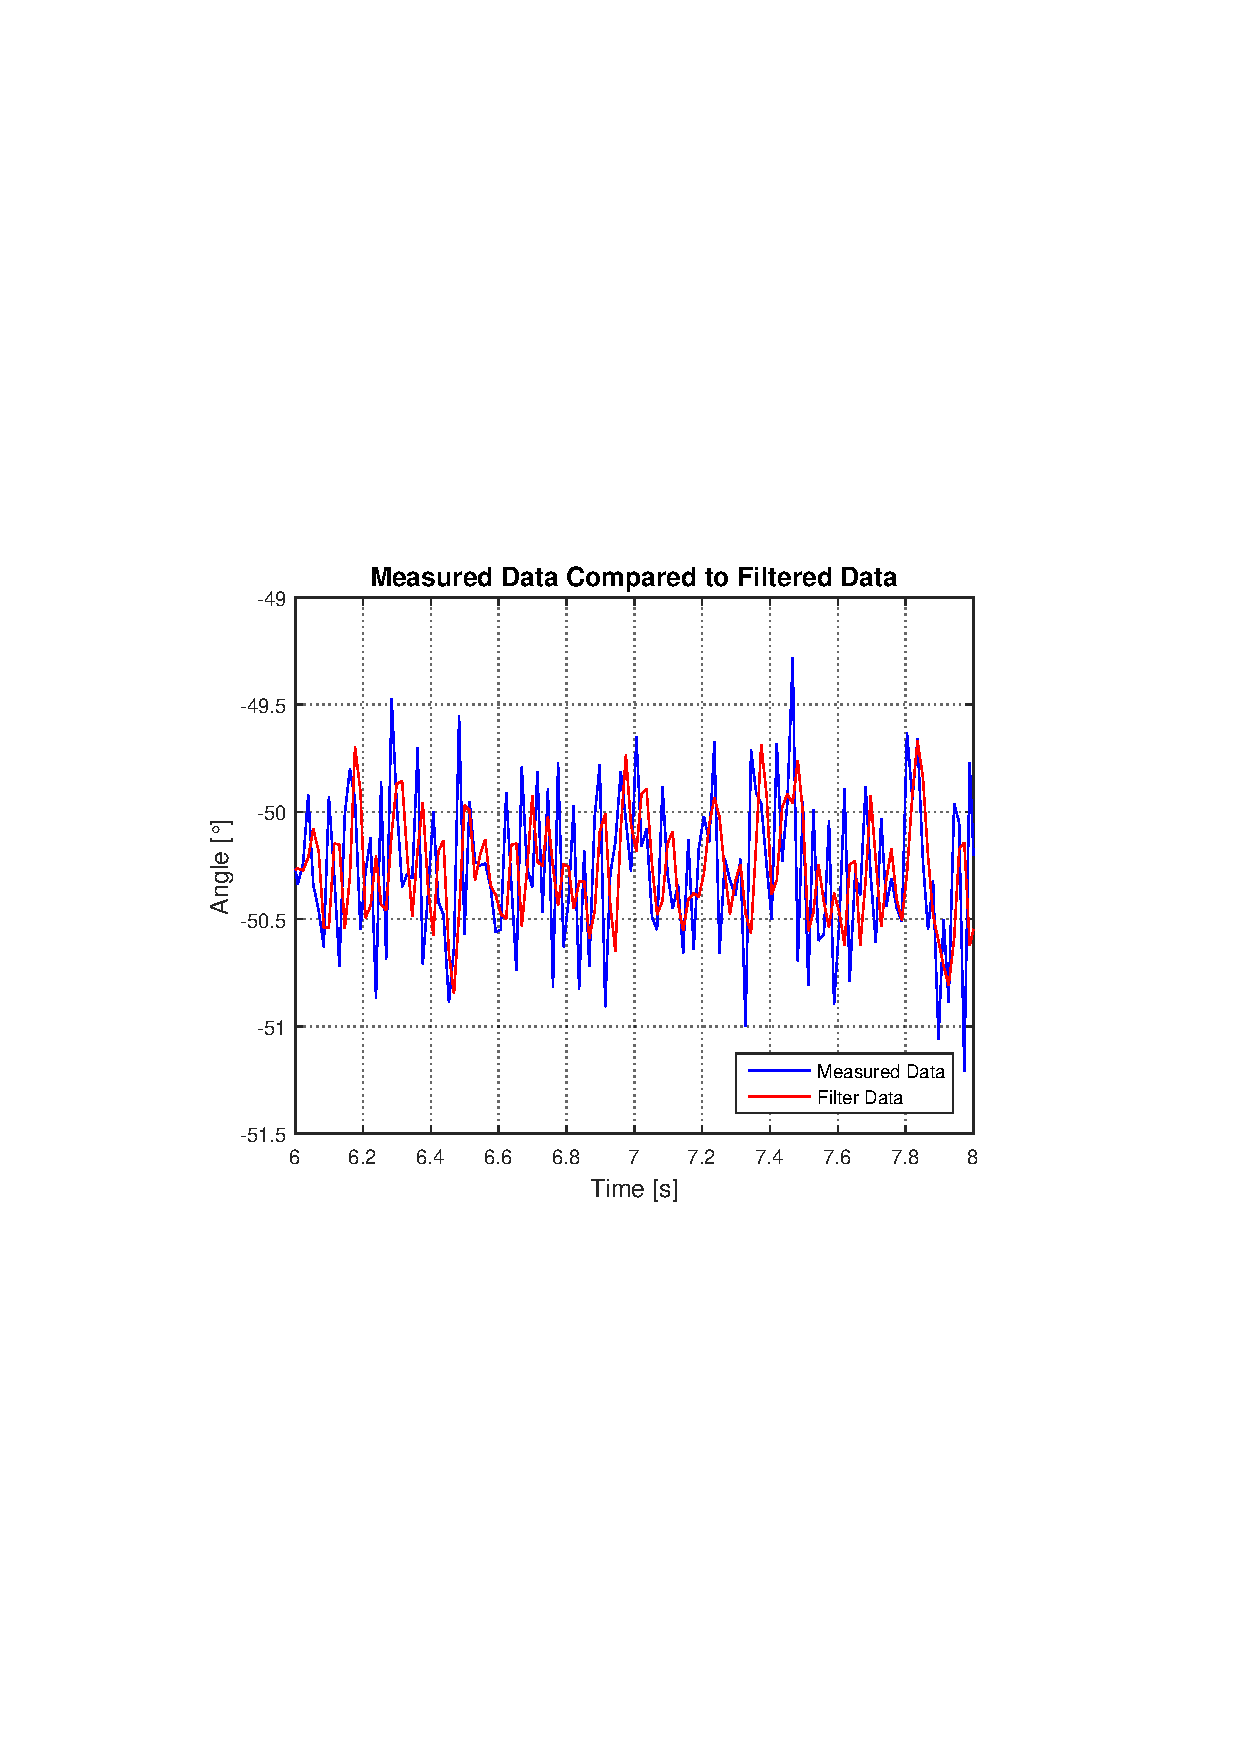
\includegraphics[width=1.2\textwidth]{figures/FinalImplementedFilter.pdf}
  }
  \caption{The original measurements from \figref{fig:StationaryMeasurementsMagnato} compared to the related measurements filtered utilizing the implemented filter in \autoref{lst:FilterMatlabImplementation}}
  \label{fig:FinalImplementedFilter}
\end{figure}

In \figref{fig:FinalImplementedFilter} the red line is the filtered data and the blue line is the raw data measured from the Magnetometer. It can be seen from the figure that the signal is still noisy, but the filter reduces the peak variations of the raw measured data, making the overall noise amplitude lower. A delay is observed, caused by the group delay in the filter.

\begin{figure}[H]
  \centering
 	%Trim margins @:   left        bottom       right       top
 	\adjustbox{ trim = {.15\width} {.30\height} {.15\width} {.30\height}, clip }
  {
    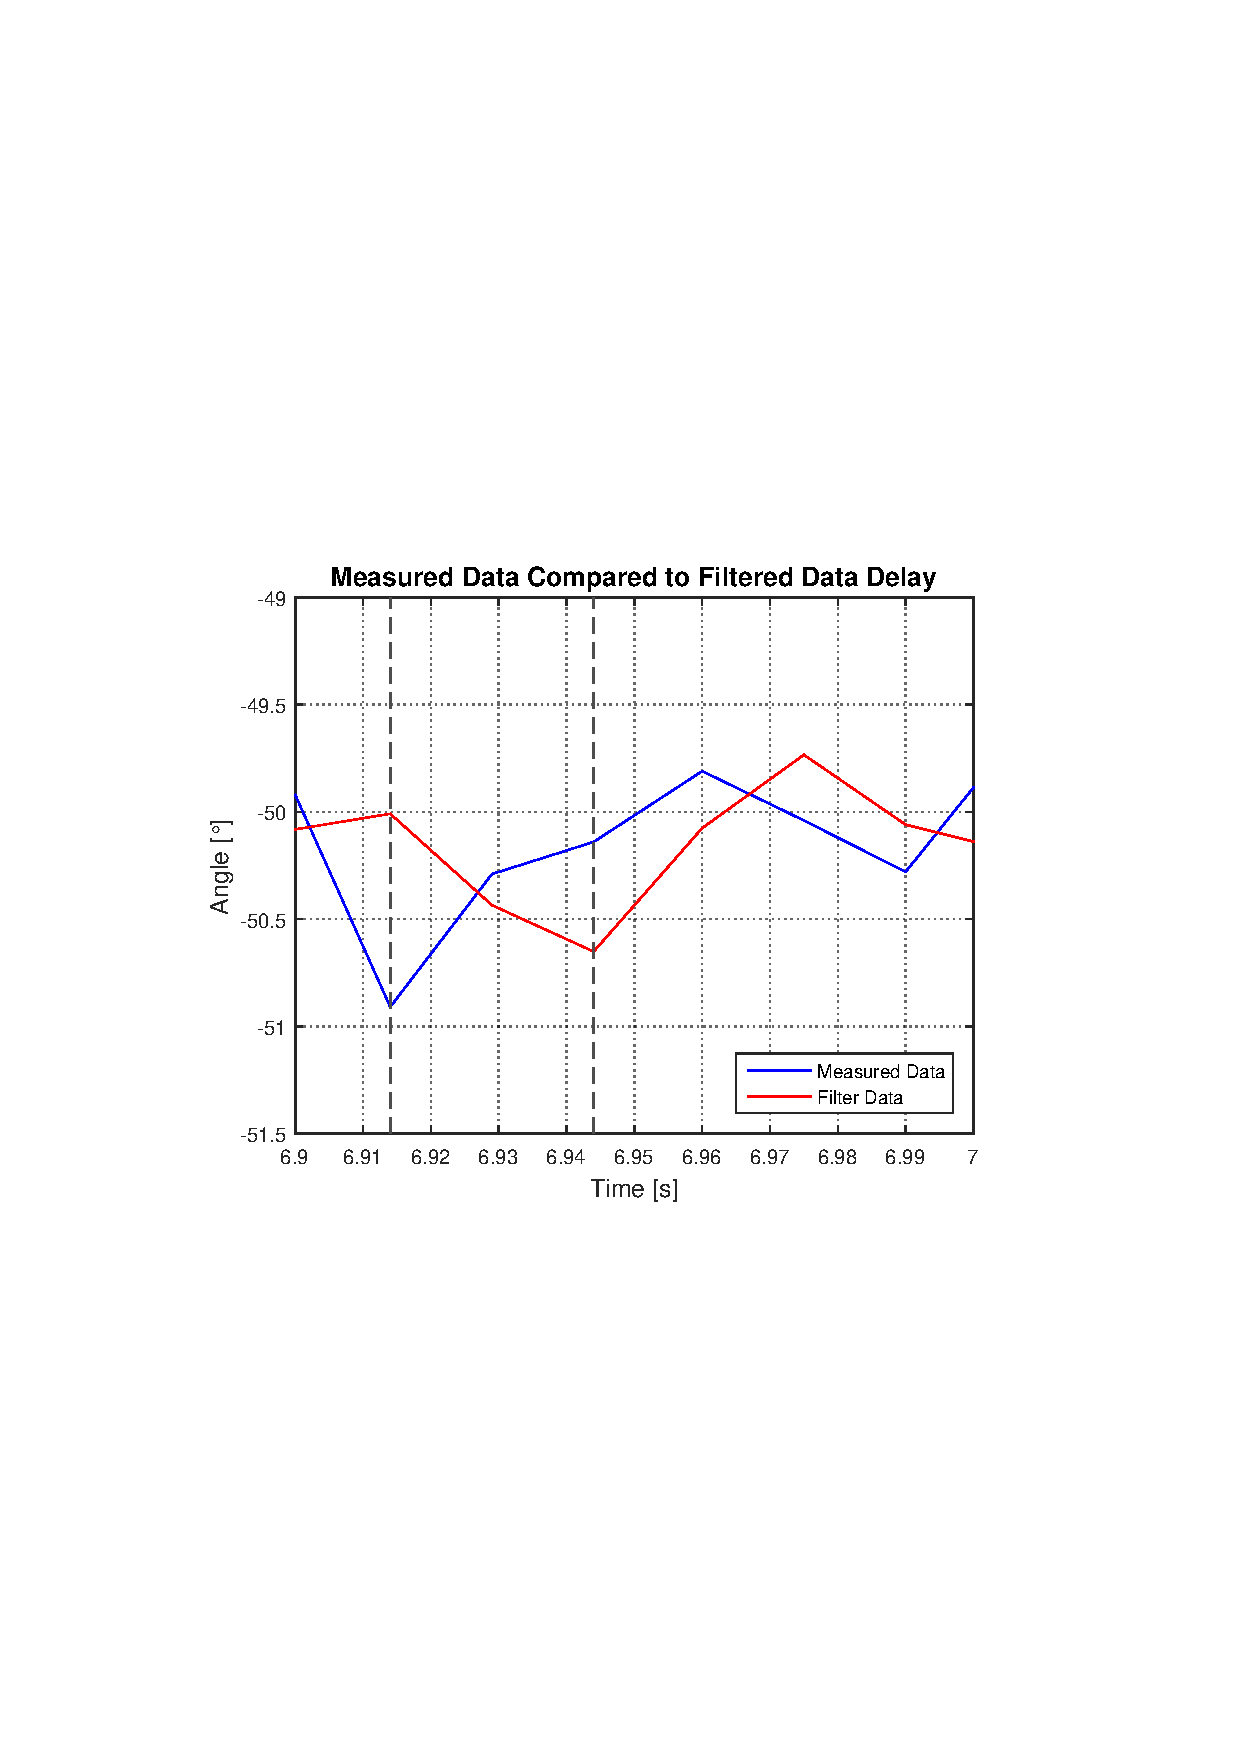
\includegraphics[width=1.2\textwidth]{figures/FinalimplementationFilterDelay.pdf}
  }
  \caption{A plot illustrating the delay occurring when the filter is implemented compared to the raw measured data received directly from the Magnetometer.}
  \label{fig:FinalimplementationFilterDelay}
\end{figure}

As seen on the figure a delay of approximately 0.03 s occurs when utilizing the filter compared to the raw measured data. If the velocity of the vehicle is 1.4 \si{\frac{m}{s}} then the vehicle will have moved approximately 4.2 \si{cm} in this time. By simulating a step response of the directional control loop with the filter, it is possible to see if the filter will make the directional control unstable. A simulation of the a step response in the directional control loop with and without filter is illustrated in \figref{fig:SimulatedStepResponsewithandwithoutFilter}.
\vspace{-10mm}{
\begin{figure}[H]
  \centering
 	%Trim margins @:   left        bottom       right       top
 	\adjustbox{ trim = {.15\width} {.315\height} {.15\width} {.30\height}, clip }
  {
    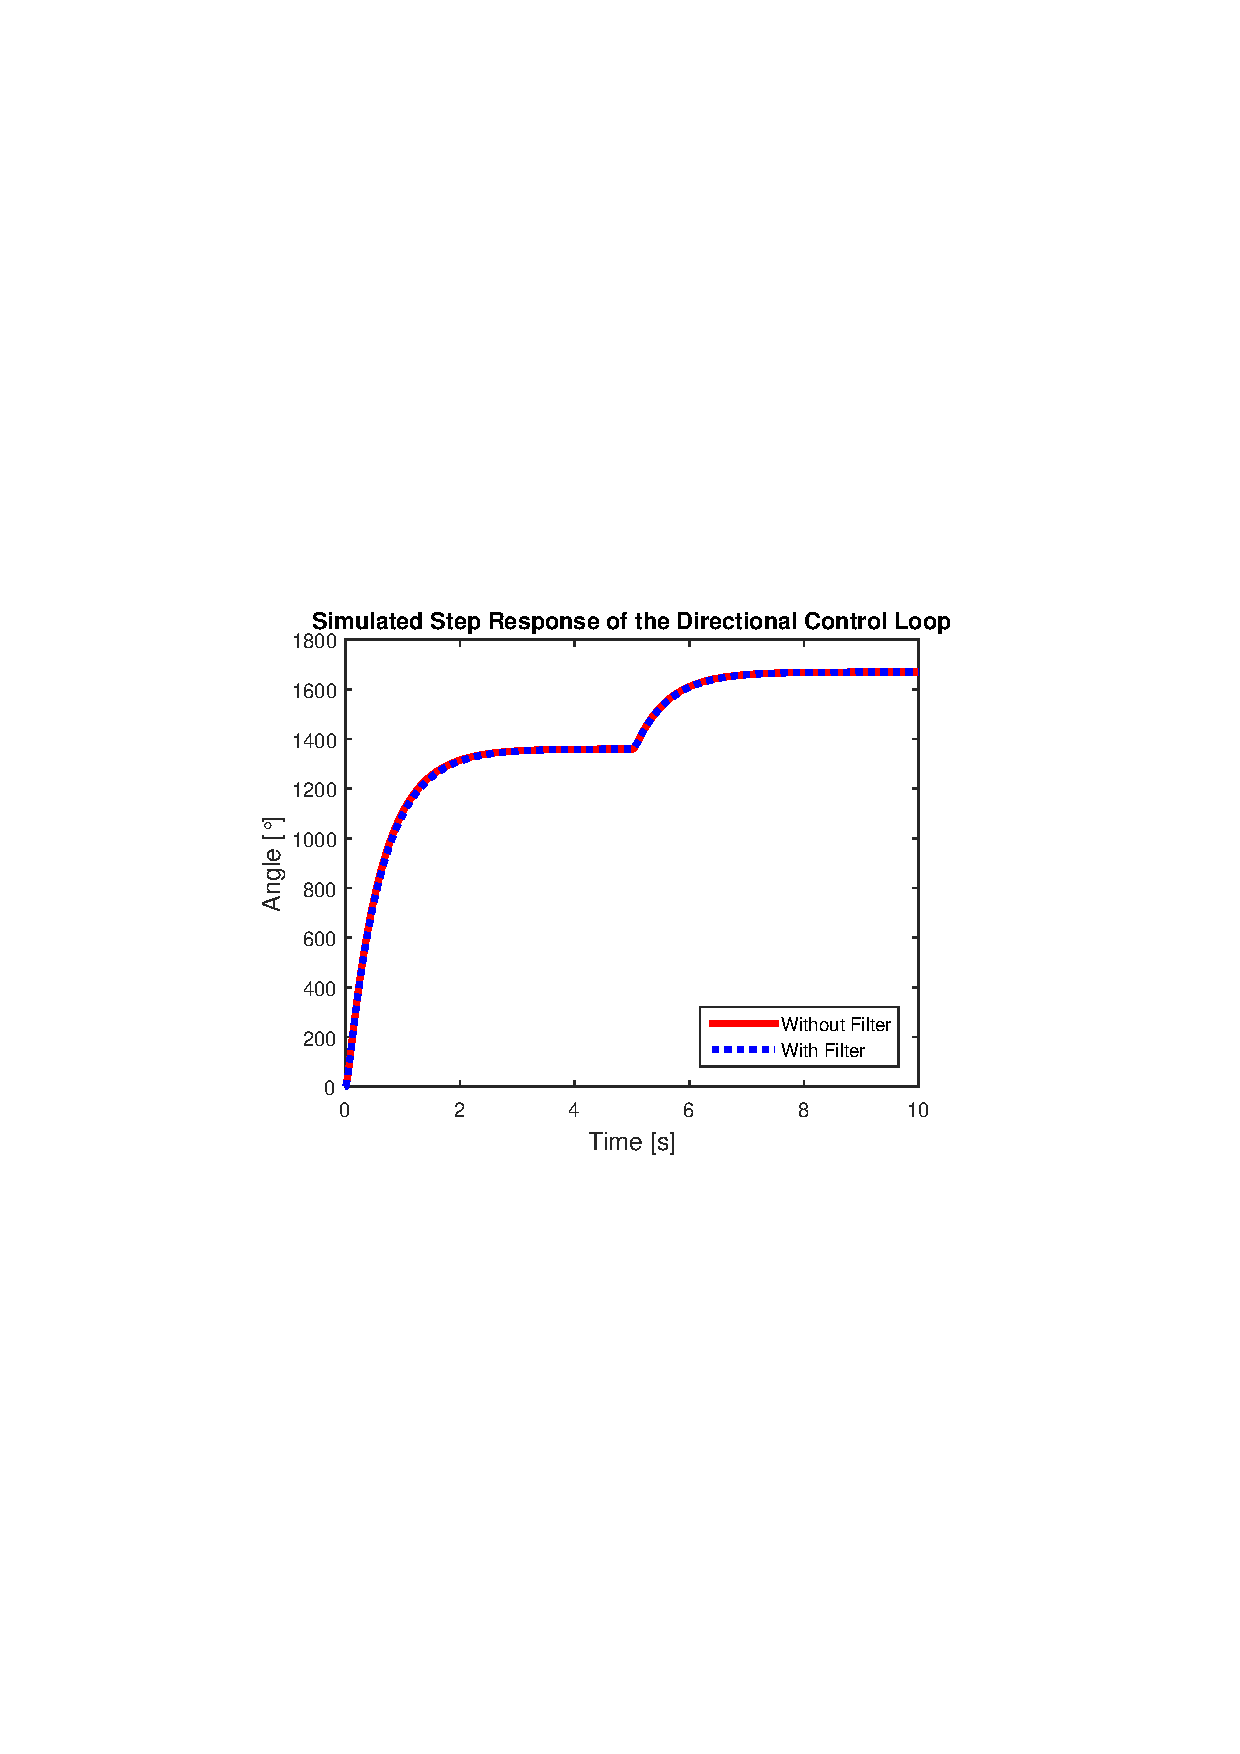
\includegraphics[width=1.2\textwidth]{figures/SimulatedStepResponsewithandwithoutFilter.pdf}
  }
  \caption{A plot illustrating a simulated step response of the directional control loop with and without the filter.}
  \label{fig:SimulatedStepResponsewithandwithoutFilter}
\end{figure}}
\vspace{-12mm}{
\begin{figure}[H]
  \centering
 	%Trim margins @:   left        bottom       right       top
 	\adjustbox{ trim = {.15\width} {.315\height} {.15\width} {.30\height}, clip }
  {
    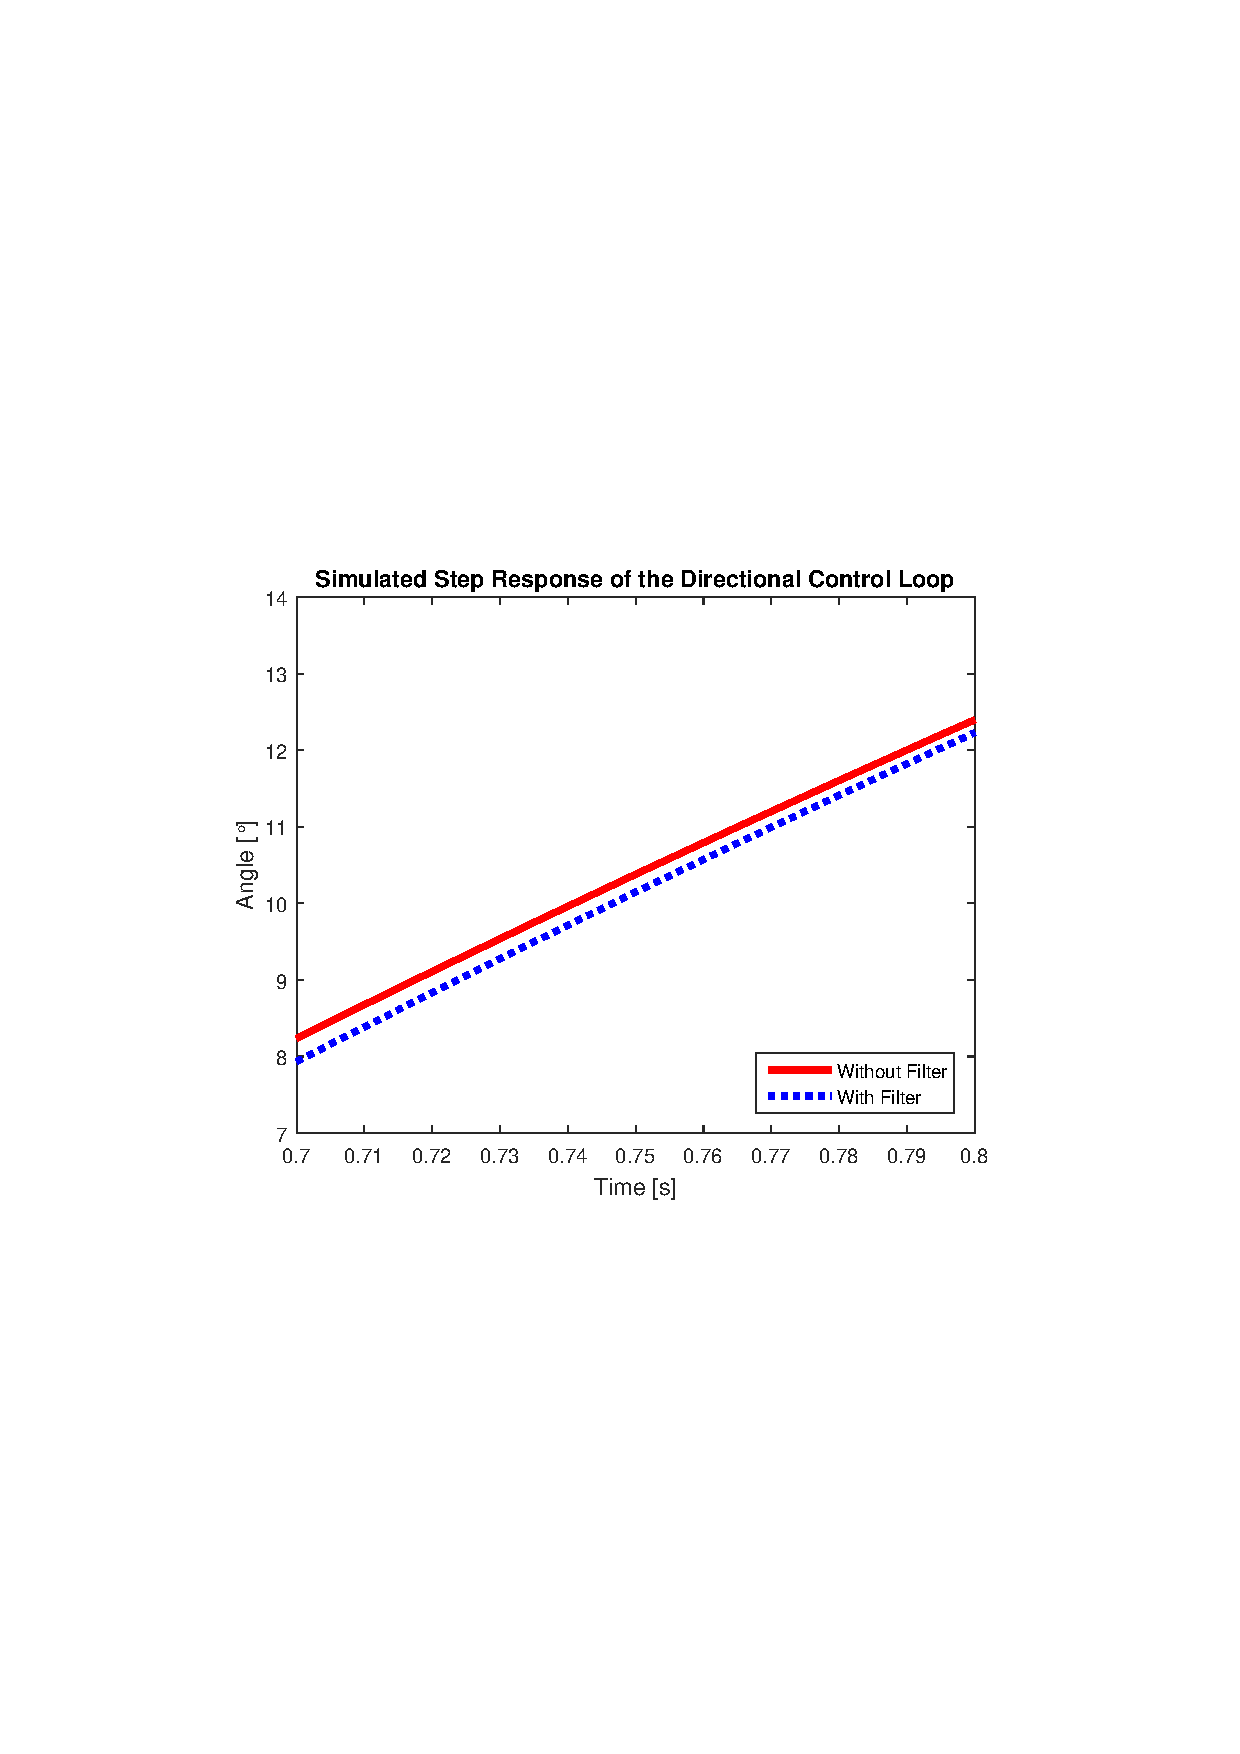
\includegraphics[width=1.2\textwidth]{figures/Withandwithoutfilterzoomed.pdf}
  }
  \caption{A zoomed in view.}
  \label{fig:Withandwithoutfilterzoomed}
\end{figure}
}
From \figref{fig:SimulatedStepResponsewithandwithoutFilter} it can be seen that the filter does not change the step response significantly. Only when zoomed in (\figref{fig:Withandwithoutfilterzoomed}), a small delay can be seen in the response.

A bode plot is now made, with and without the filter, see \figref{{fig:IIRfilter}}.

\begin{figure}[H]
	\centering
	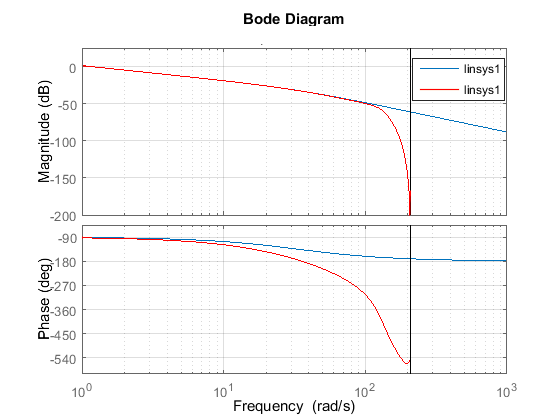
\includegraphics[scale=1]{figures/2xBode.png}
	\caption{Open loop Bode plot of the angular controller, with(red) and without(blue) the IIR filter}
	\label{fig:IIRfilter}
\end{figure}

As seen on the bode plot, the filter does not affect the magnitude response of the system until around 100 rad/s. The phase remains close until around 10 rad/s, and then starts to deviate. This frequency is well above the dominant pole, which explains why the step response remains nearly unchanged. As the filter introduces 4 extra poles, the total phase shift is expected to be $4\cdot 90^\circ = 360^\circ$ larger, which is confirmed. As the loop has no gain, stability is ensured.

While the filter has been verified to be functional, without affecting the stability of the system, the results are not convincing. While the bode plots looks nice, and the largest peaks of the noise have been removed, the noise looks close to unchanged (\figref{fig:FinalImplementedFilter}). As the microcontroller has no floating point calculation hardware, the filter will be expensive in processing time, with very little improvements in return. Considering this, the filter will not be implemented.
